\section{Presentation Logic Layer}

%What pages will be present in your project? briefly indicate how your web site will be organized

The website will be divided into the following pages:
\begin{itemize}
    \item Login page: allows the users login to the web application. 
    User must enter their email or username and password for account authentication.
    \item Sign up page: allows the user to register to the web pages. 
    The registration process is divided into 3 different steps/pages where different
    info are requested.
    \begin{itemize}
        \item Personal information page: asks for the user's name, surname, role, brand name, birth date and a recommended profile image.
        \item Address information page: asks for the user's address, city, country and post code.
        \item Account information page: asks to insert the username, email and password for the account.
    \end{itemize}
    \item Homepage: shows the most recent art pieces uploaded by the artists the logged user is following. 
    Also allows user to follow new artists by searching them by username.
    \item Profile settings page: allows user to edit their account info and to access their order history and following lists, which are shown in separate pages.
    \item Artist profile page: is a space managed by an artist where his/her info are shown. 
    Is divided into 3 sections:
    \begin{itemize}
        \item Showcase section: accessed by other users to see a complete list of the artist uploaded art pieces.
        \item Shop section: accessed by other users to potentially buy an art piece being sold by the artist.
        \item Biography section: accessed by other users to get to know more about the artist the profile belongs to.
    \end{itemize}
    \item Art gallery profile page: is similar to the previous described page, but it has only two sections:
    \begin{itemize}
        \item Showcase section: accessed by other users to see the events held in the art gallery.
        \item Biography section: accessed by other users to get to know more about the art gallery the profile belongs to.
    \end{itemize}
    \item Art piece page: displays additional info about an art piece. If it is being sold also allows access to a buy option, which leads to the order page.
    \item Order page: allows the user to buy an art piece. The user will se a summary of the order and will be asked to pay using his PayPal account.
    \item Order history page: shows the user's order history. To simplify the search for a specific order, the user can filter the orders by date or cost. 
\end{itemize}

Except for the login and sign up pages, every page within the web application features a persistent side navigation bar that enhances overall usability. 
This component provides quick access to essential sections such as the homepage, notifications, settings, and the user’s profile.

%%%%%%%%%%%%%%%%%%%%%%%%%%%%%%%%%%%%%%%%%%%%%%%%%%%%%%%
% Define a variable for the figure width. You can adjust this value to change all figures.
\newcommand{\myfigwidth}{0.47\textwidth}

\subsection{Login page (Interface Mokups)}
\begin{figure}[H]
    \centering
    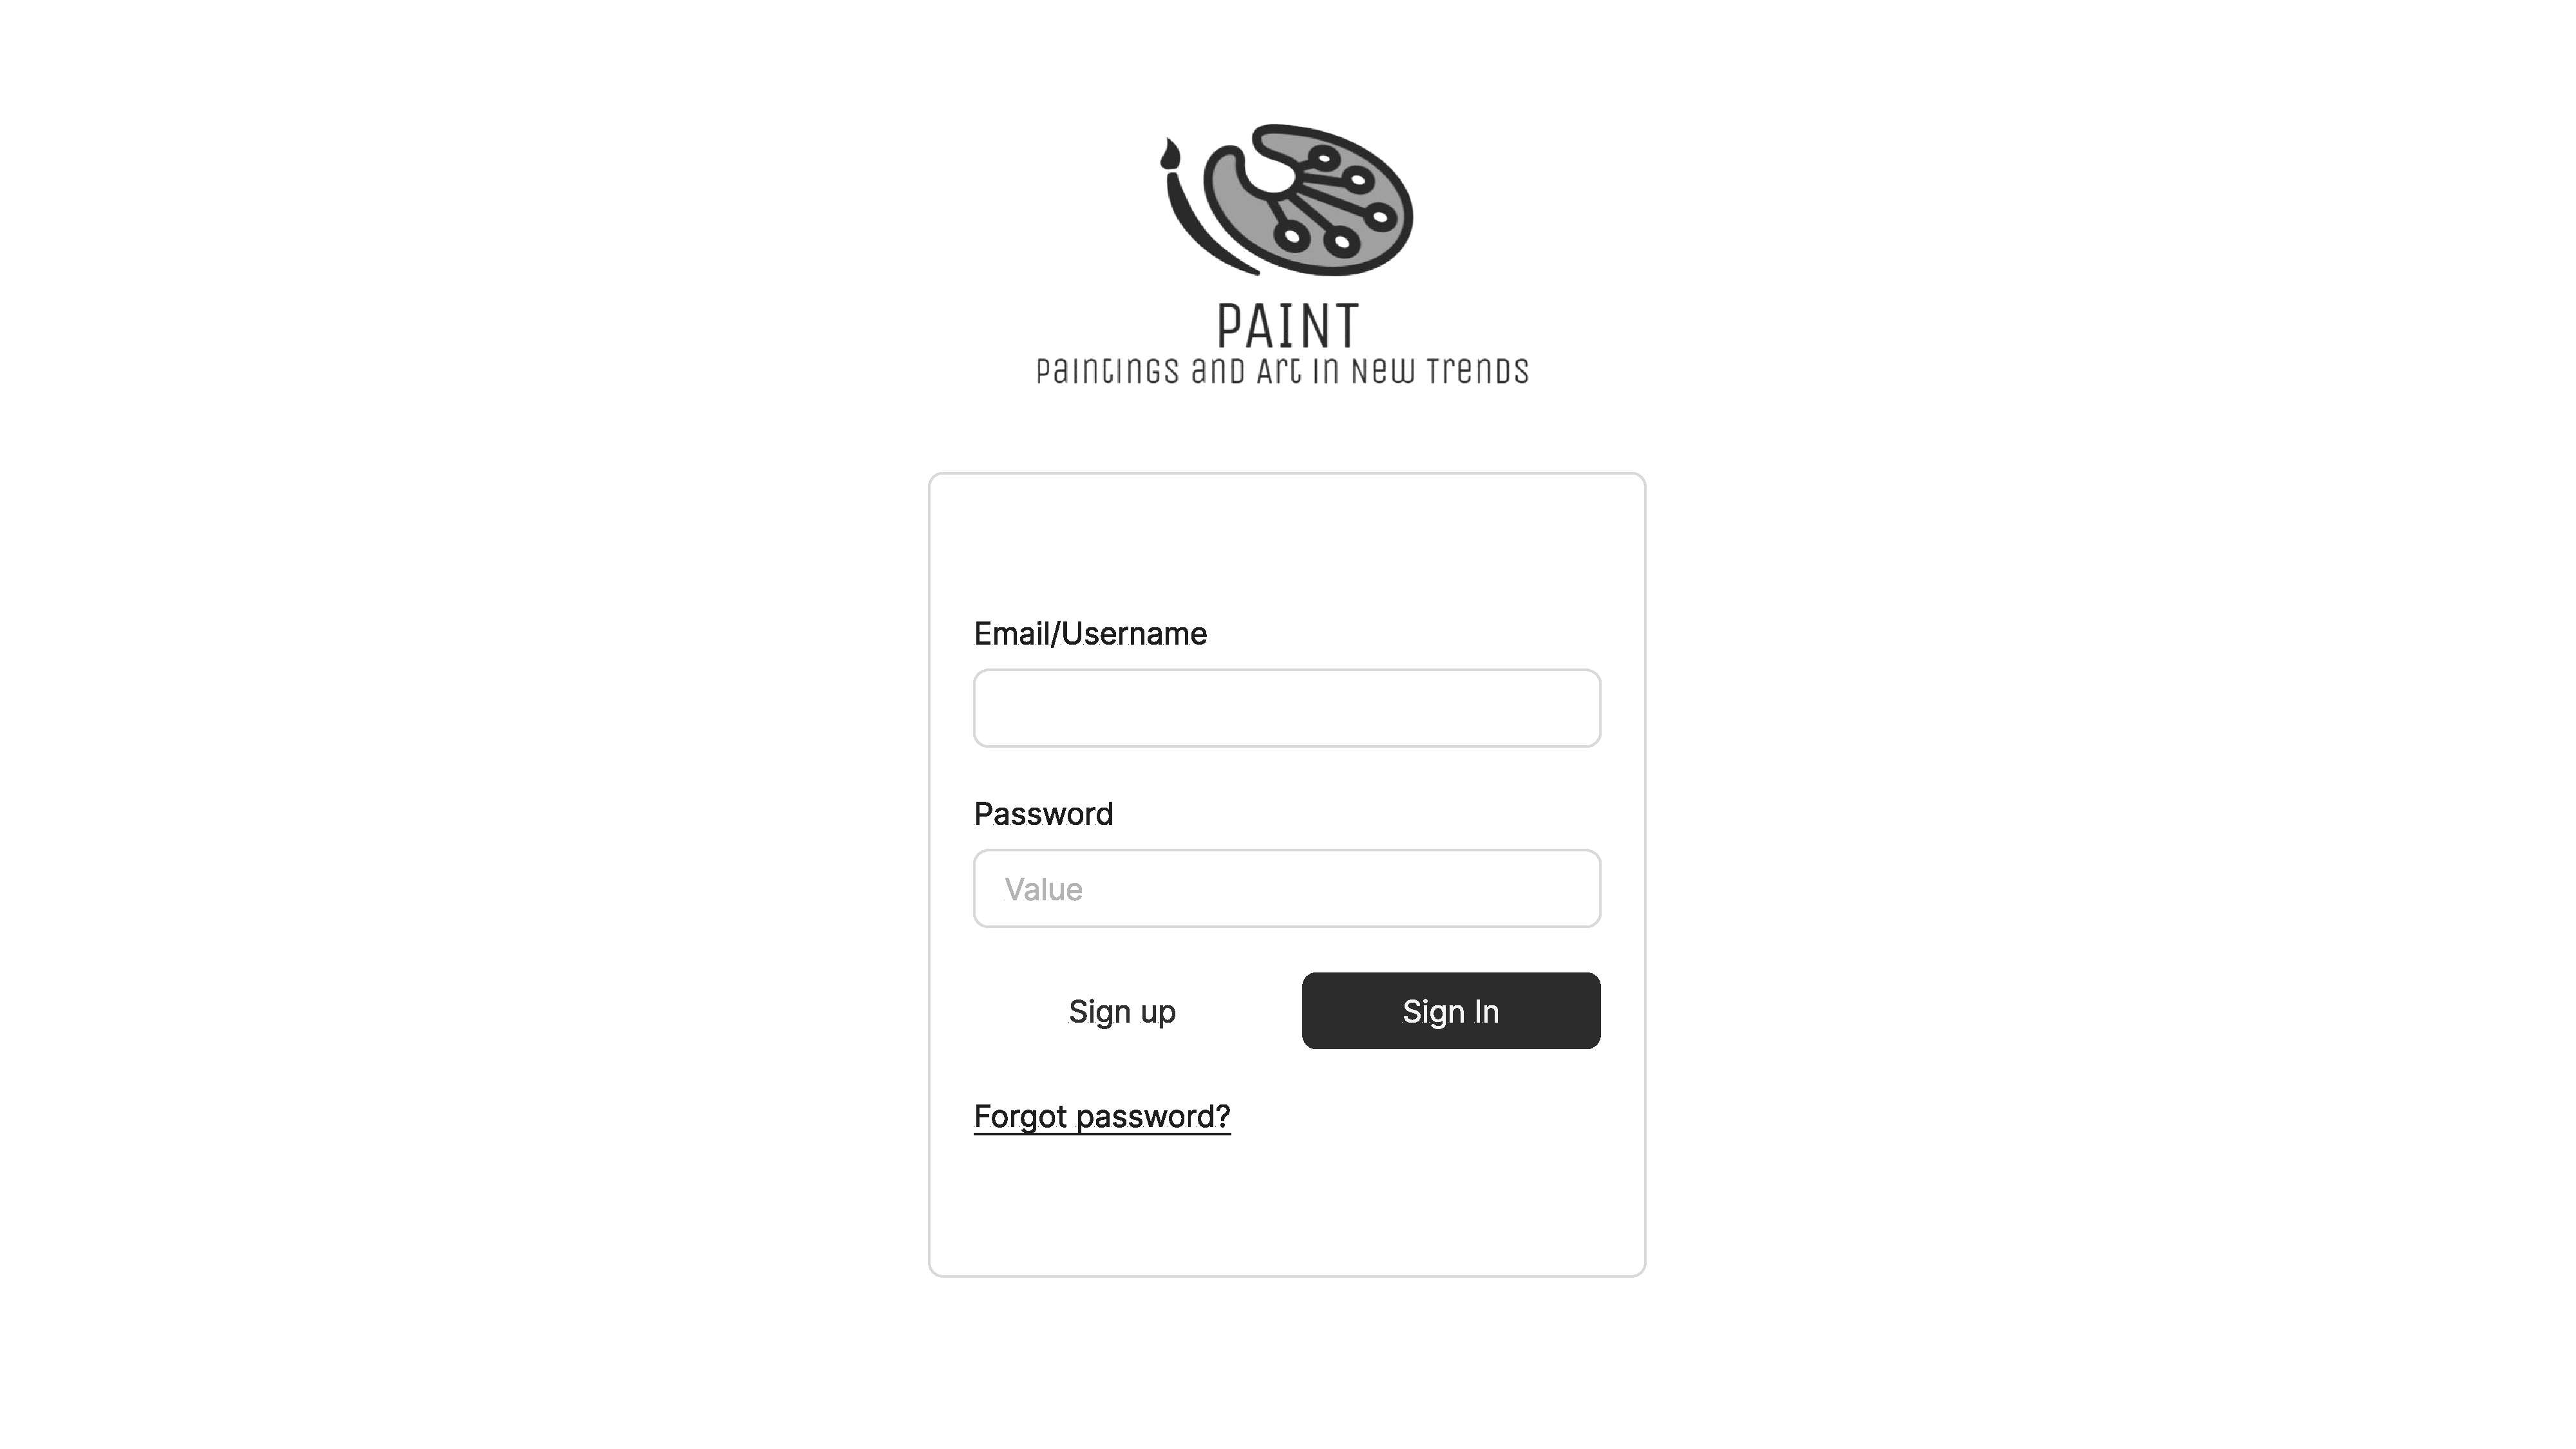
\includegraphics[width=\myfigwidth]{images/interface_mockups/Landing page - login.pdf}
    \caption{Login page}
\end{figure}

The login page is designed to authenticate users by requesting their email and password to access the web application. 
If a user forgets their password, they have the option to request a reset link, which will be sent to their registered email. 
Upon submission, the system validates the credentials against the stored records, granting access if they comply with the security standards. 
In the event of incorrect credentials, an informative error message is displayed, prompting users to re-enter their details. 
Once successfully logged in, users are redirected to the homepage.

%%%%%%%%%%%%%%%%%%%%%%%%%%%%%%%%%%%%%%%%%%%%%%%%%%%%%%%
\subsection{Signup page (Interface Mokup)}
\begin{figure}[H]
    \centering
\begin{subfigure}[b]{\myfigwidth}
    \centering
    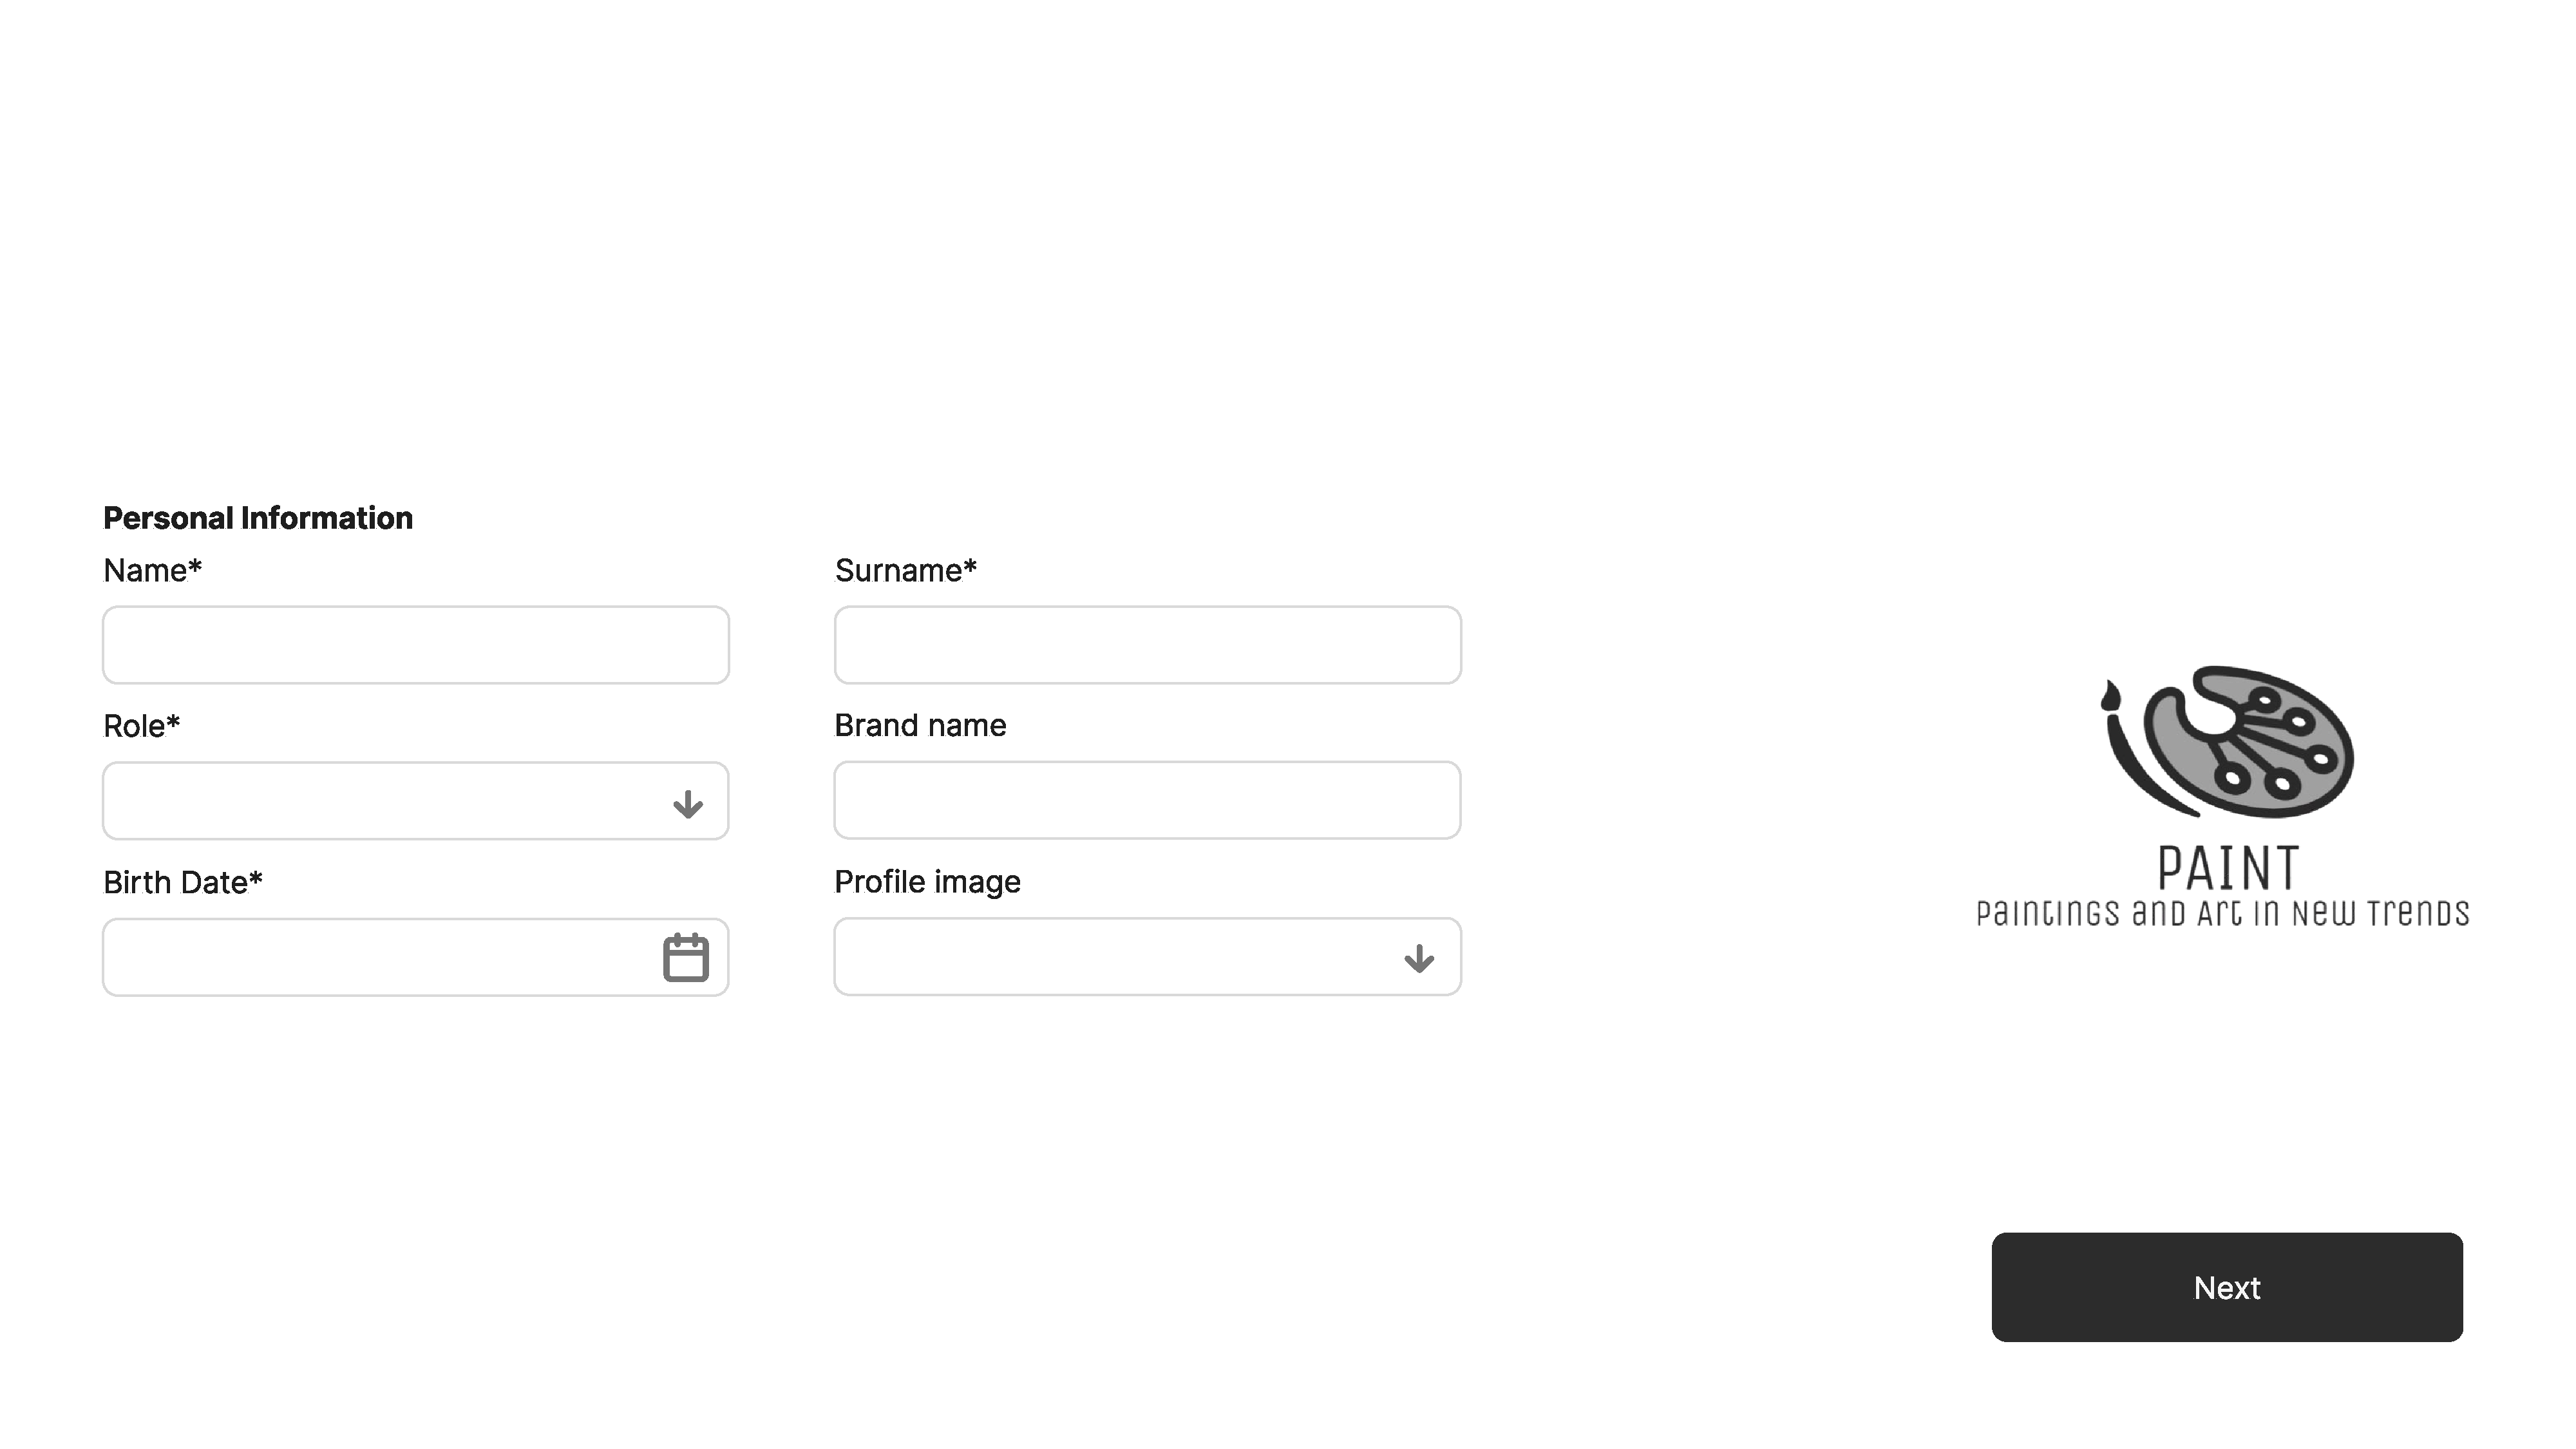
\includegraphics[width=\textwidth]{images/interface_mockups/Landing page - sign up - personal information.pdf}
    \caption{Personal information page}
\end{subfigure}
\begin{subfigure}[b]{\myfigwidth}
    \centering
    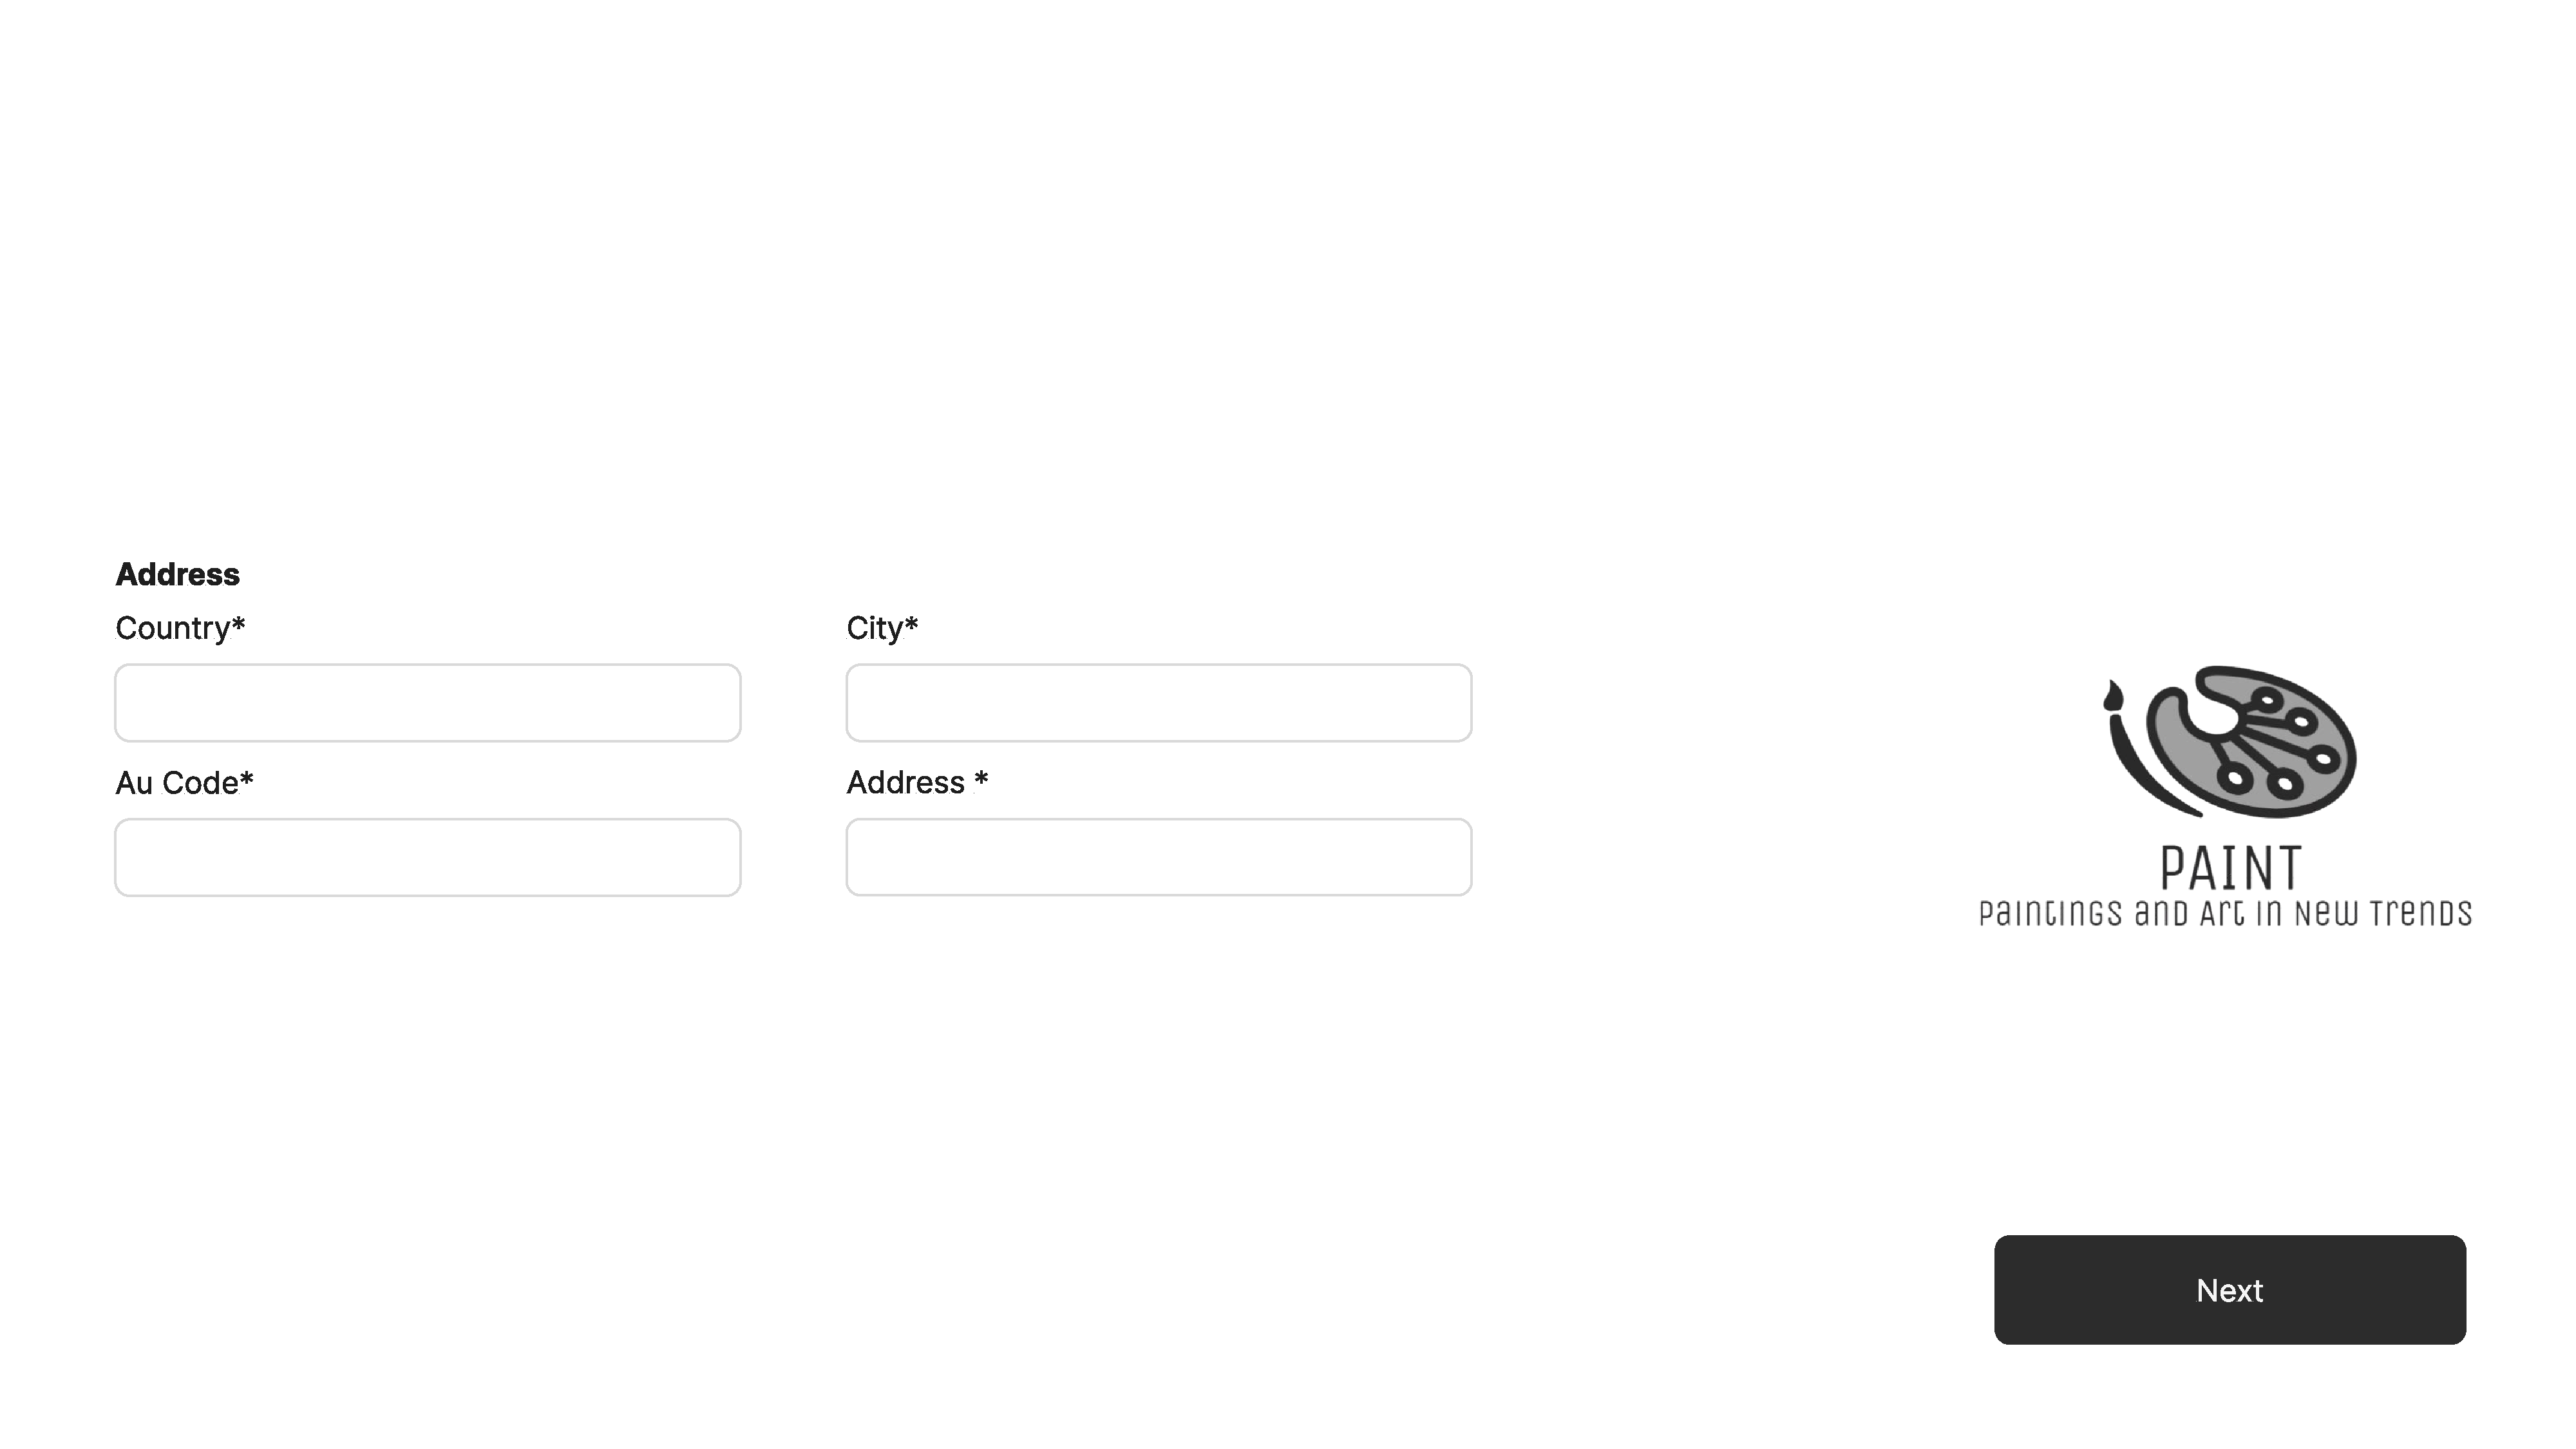
\includegraphics[width=\textwidth]{images/interface_mockups/Landing page - sign up - address information.pdf}
    \caption{Address information page}
\end{subfigure}
\begin{subfigure}[b]{\myfigwidth}
    \centering
    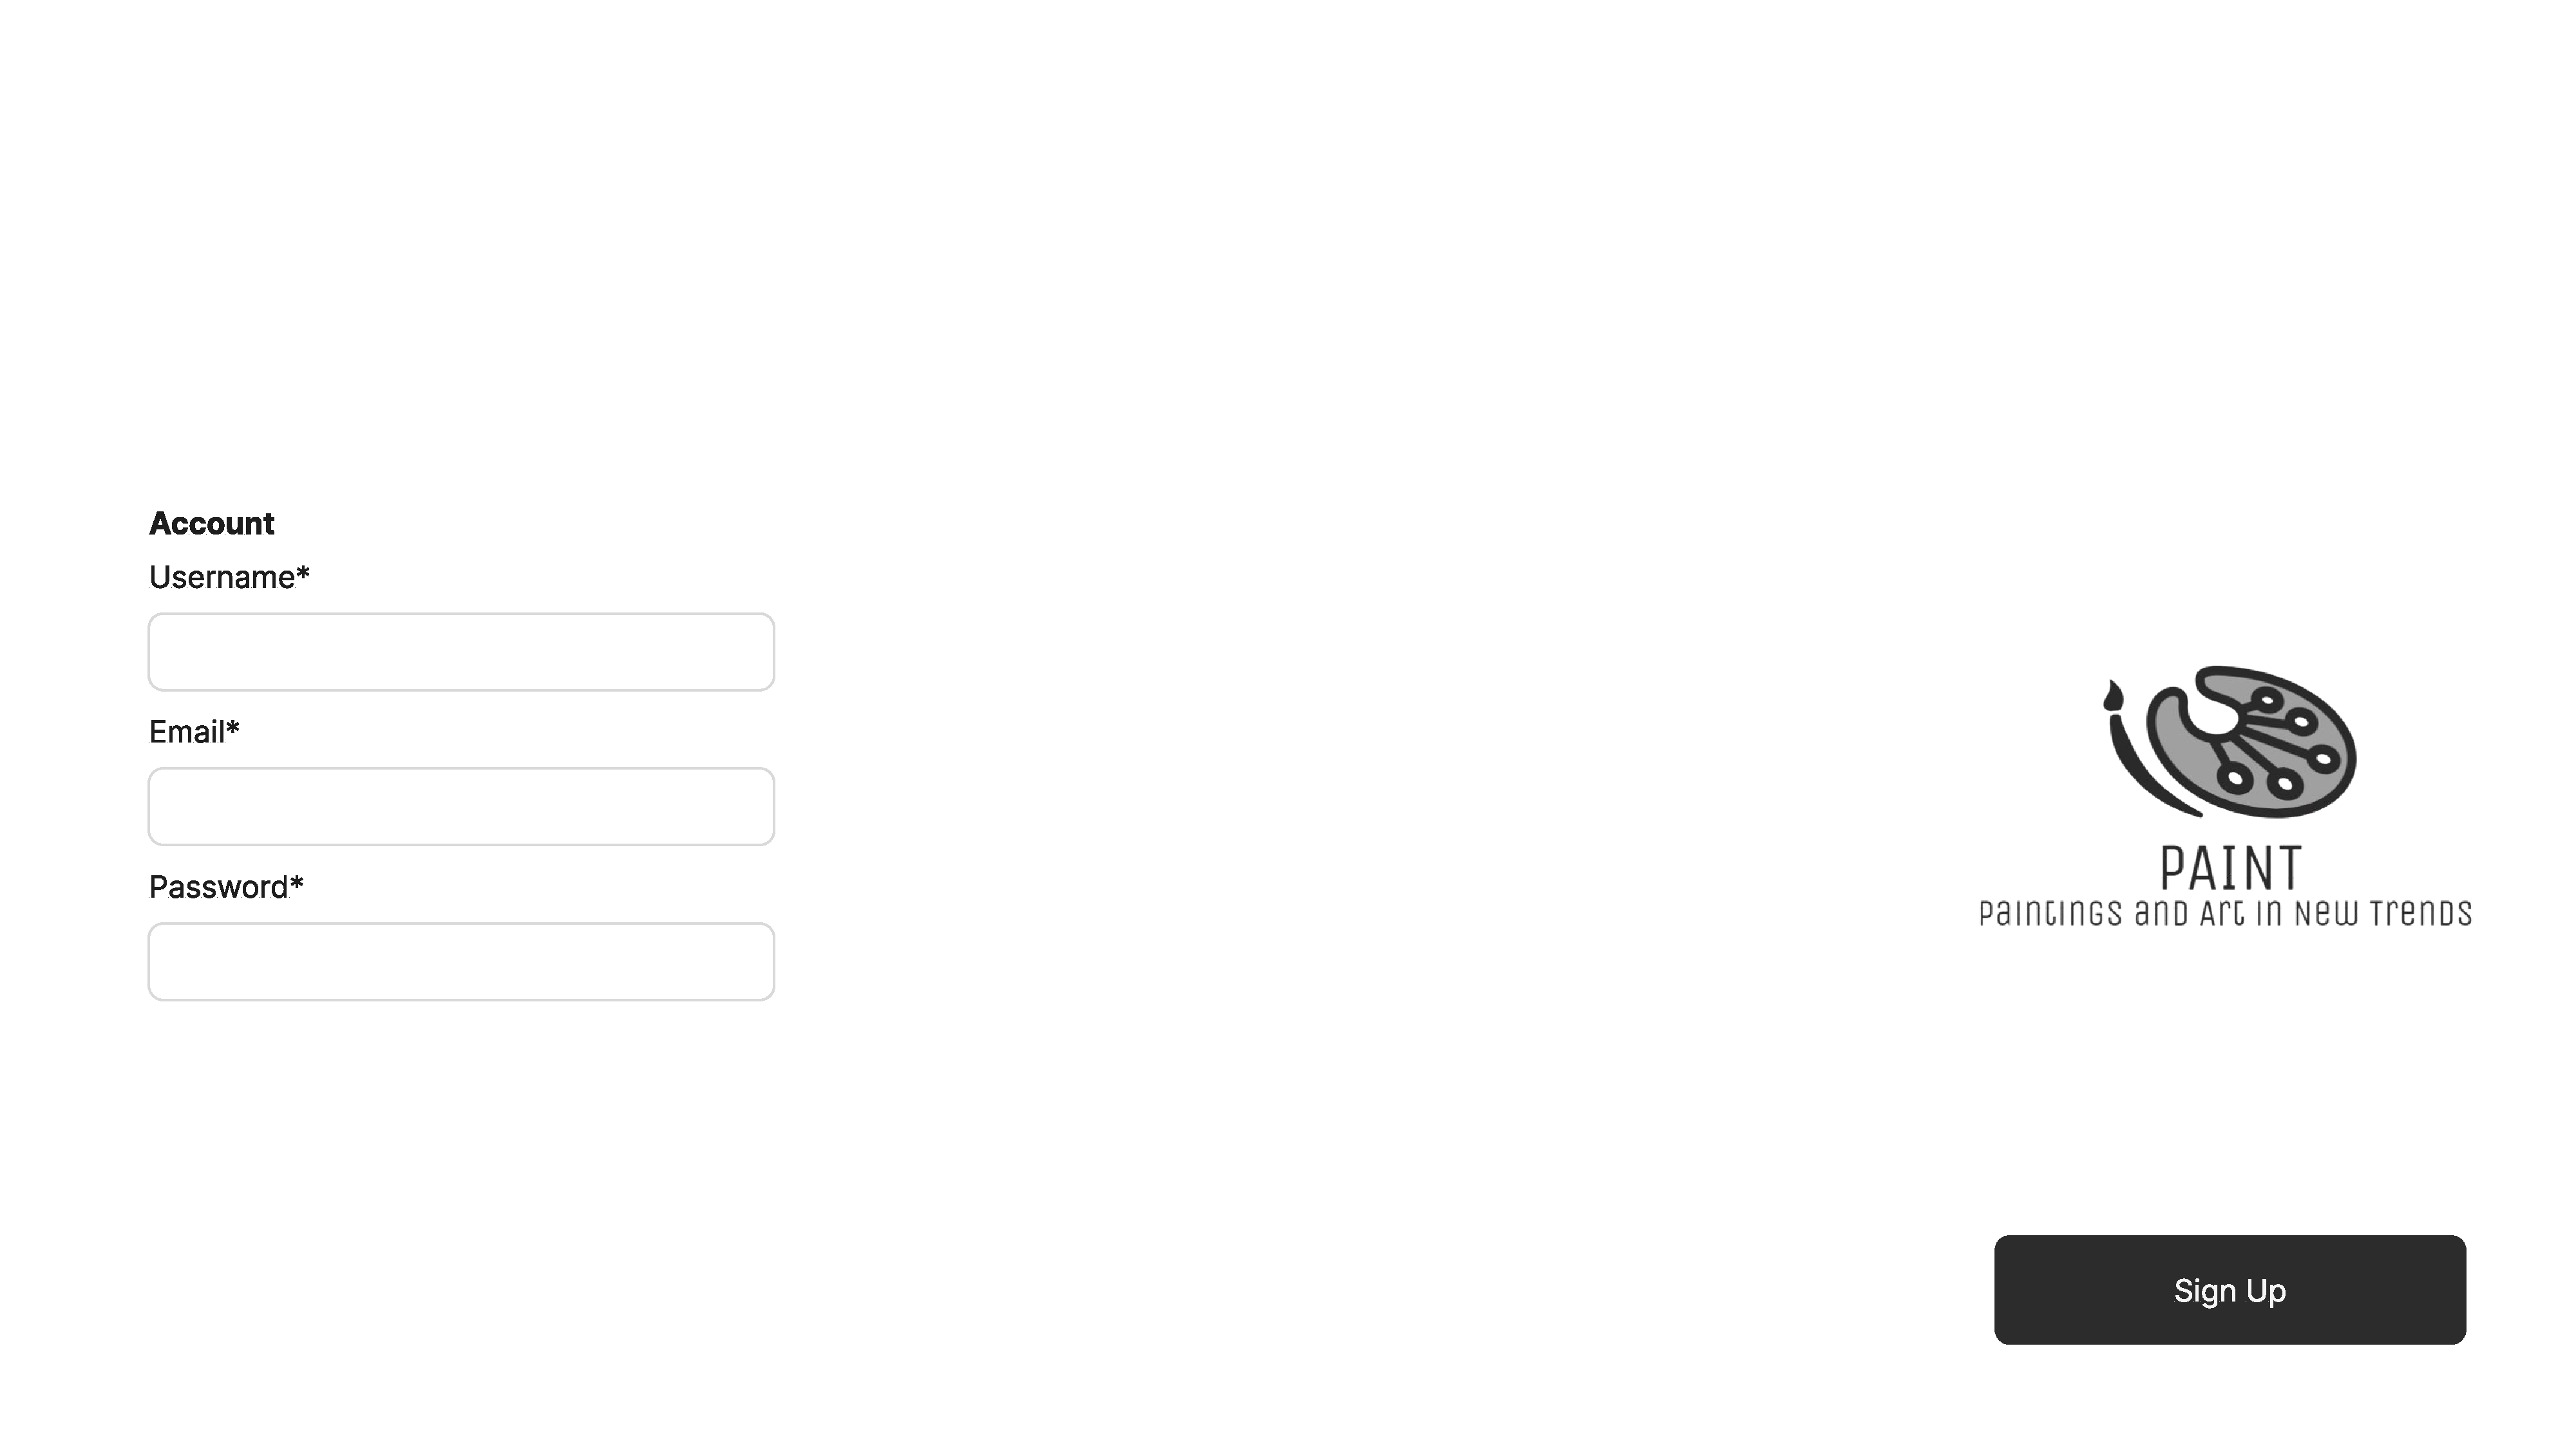
\includegraphics[width=\textwidth]{images/interface_mockups/Landing page - sign up - account information.pdf}
    \caption{Account information page}
\end{subfigure}
\end{figure}


The registration process is divided into three steps to collect detailed user information. 
In the first step, users provide their personal information, including name, surname, role, date of birth, and an optional profile image. If the selected role is 'Art gallery' or 'Business user', the user is required to insert the Brand name. 
The second step collects address details such as street address, city, country, and postal code. 
In the final step, users create their account by selecting a unique username, providing an email, and setting a password that meets security requirements.
By clicking the "Sign up" button, the user's information is validated and stored in the database.
Upon successful registration, users are redirected to the login page to access their new account.

%%%%%%%%%%%%%%%%%%%%%%%%%%%%%%%%%%%%%%%%%%%%%%%%%%%%%%%
\subsection{Homepage (Interface Mokup)}
\begin{figure}[H]
    \centering
    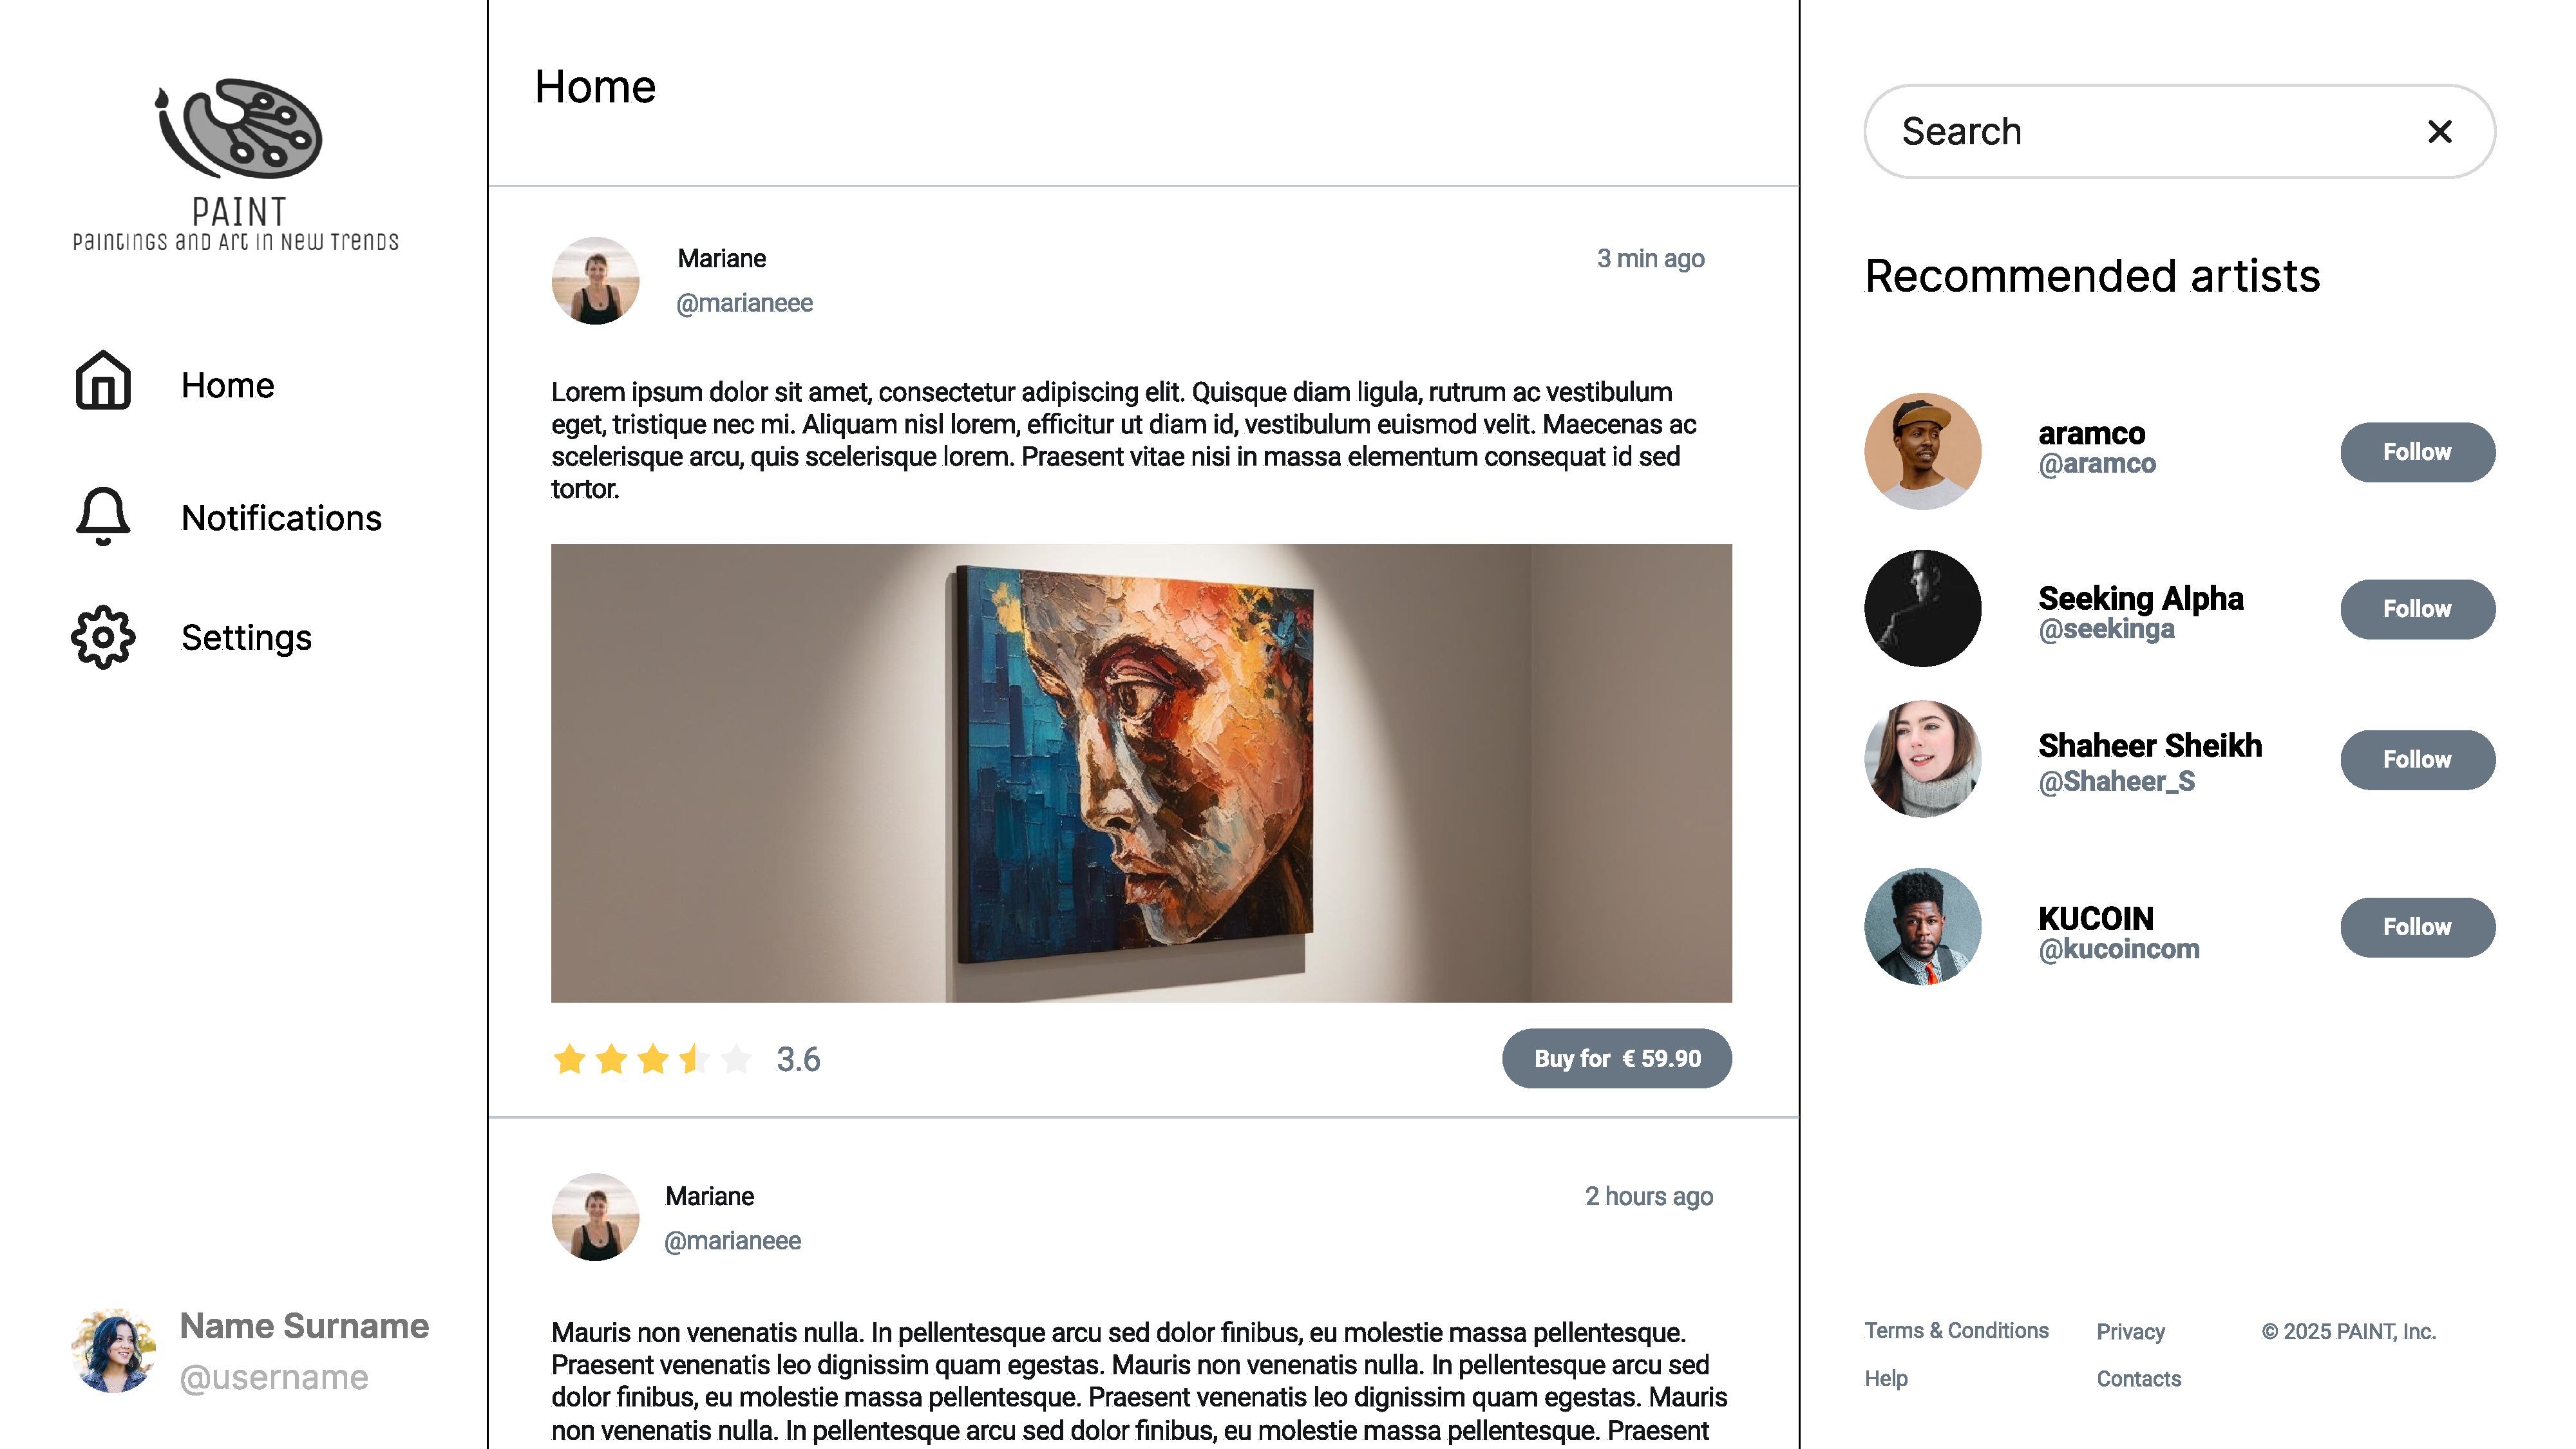
\includegraphics[width=\myfigwidth]{images/interface_mockups/Home - regular users.pdf}
    \caption{Homepage for regular users}
\end{figure}

The homepage functions as the central hub for authenticated users, showcasing the most recent art pieces uploaded by the artists and art galleries they follow.
Users can also search for new artists by their username and follow them. 
On the right, users can see popular profiles on the platform and quickly follow them.

%%%%%%%%%%%%%%%%%%%%%%%%%%%%%%%%%%%%%%%%%%%%%%%%%%%%%%%
\subsection{Profile settings page (Interface Mokup)}
\begin{figure}[H]
    \centering
    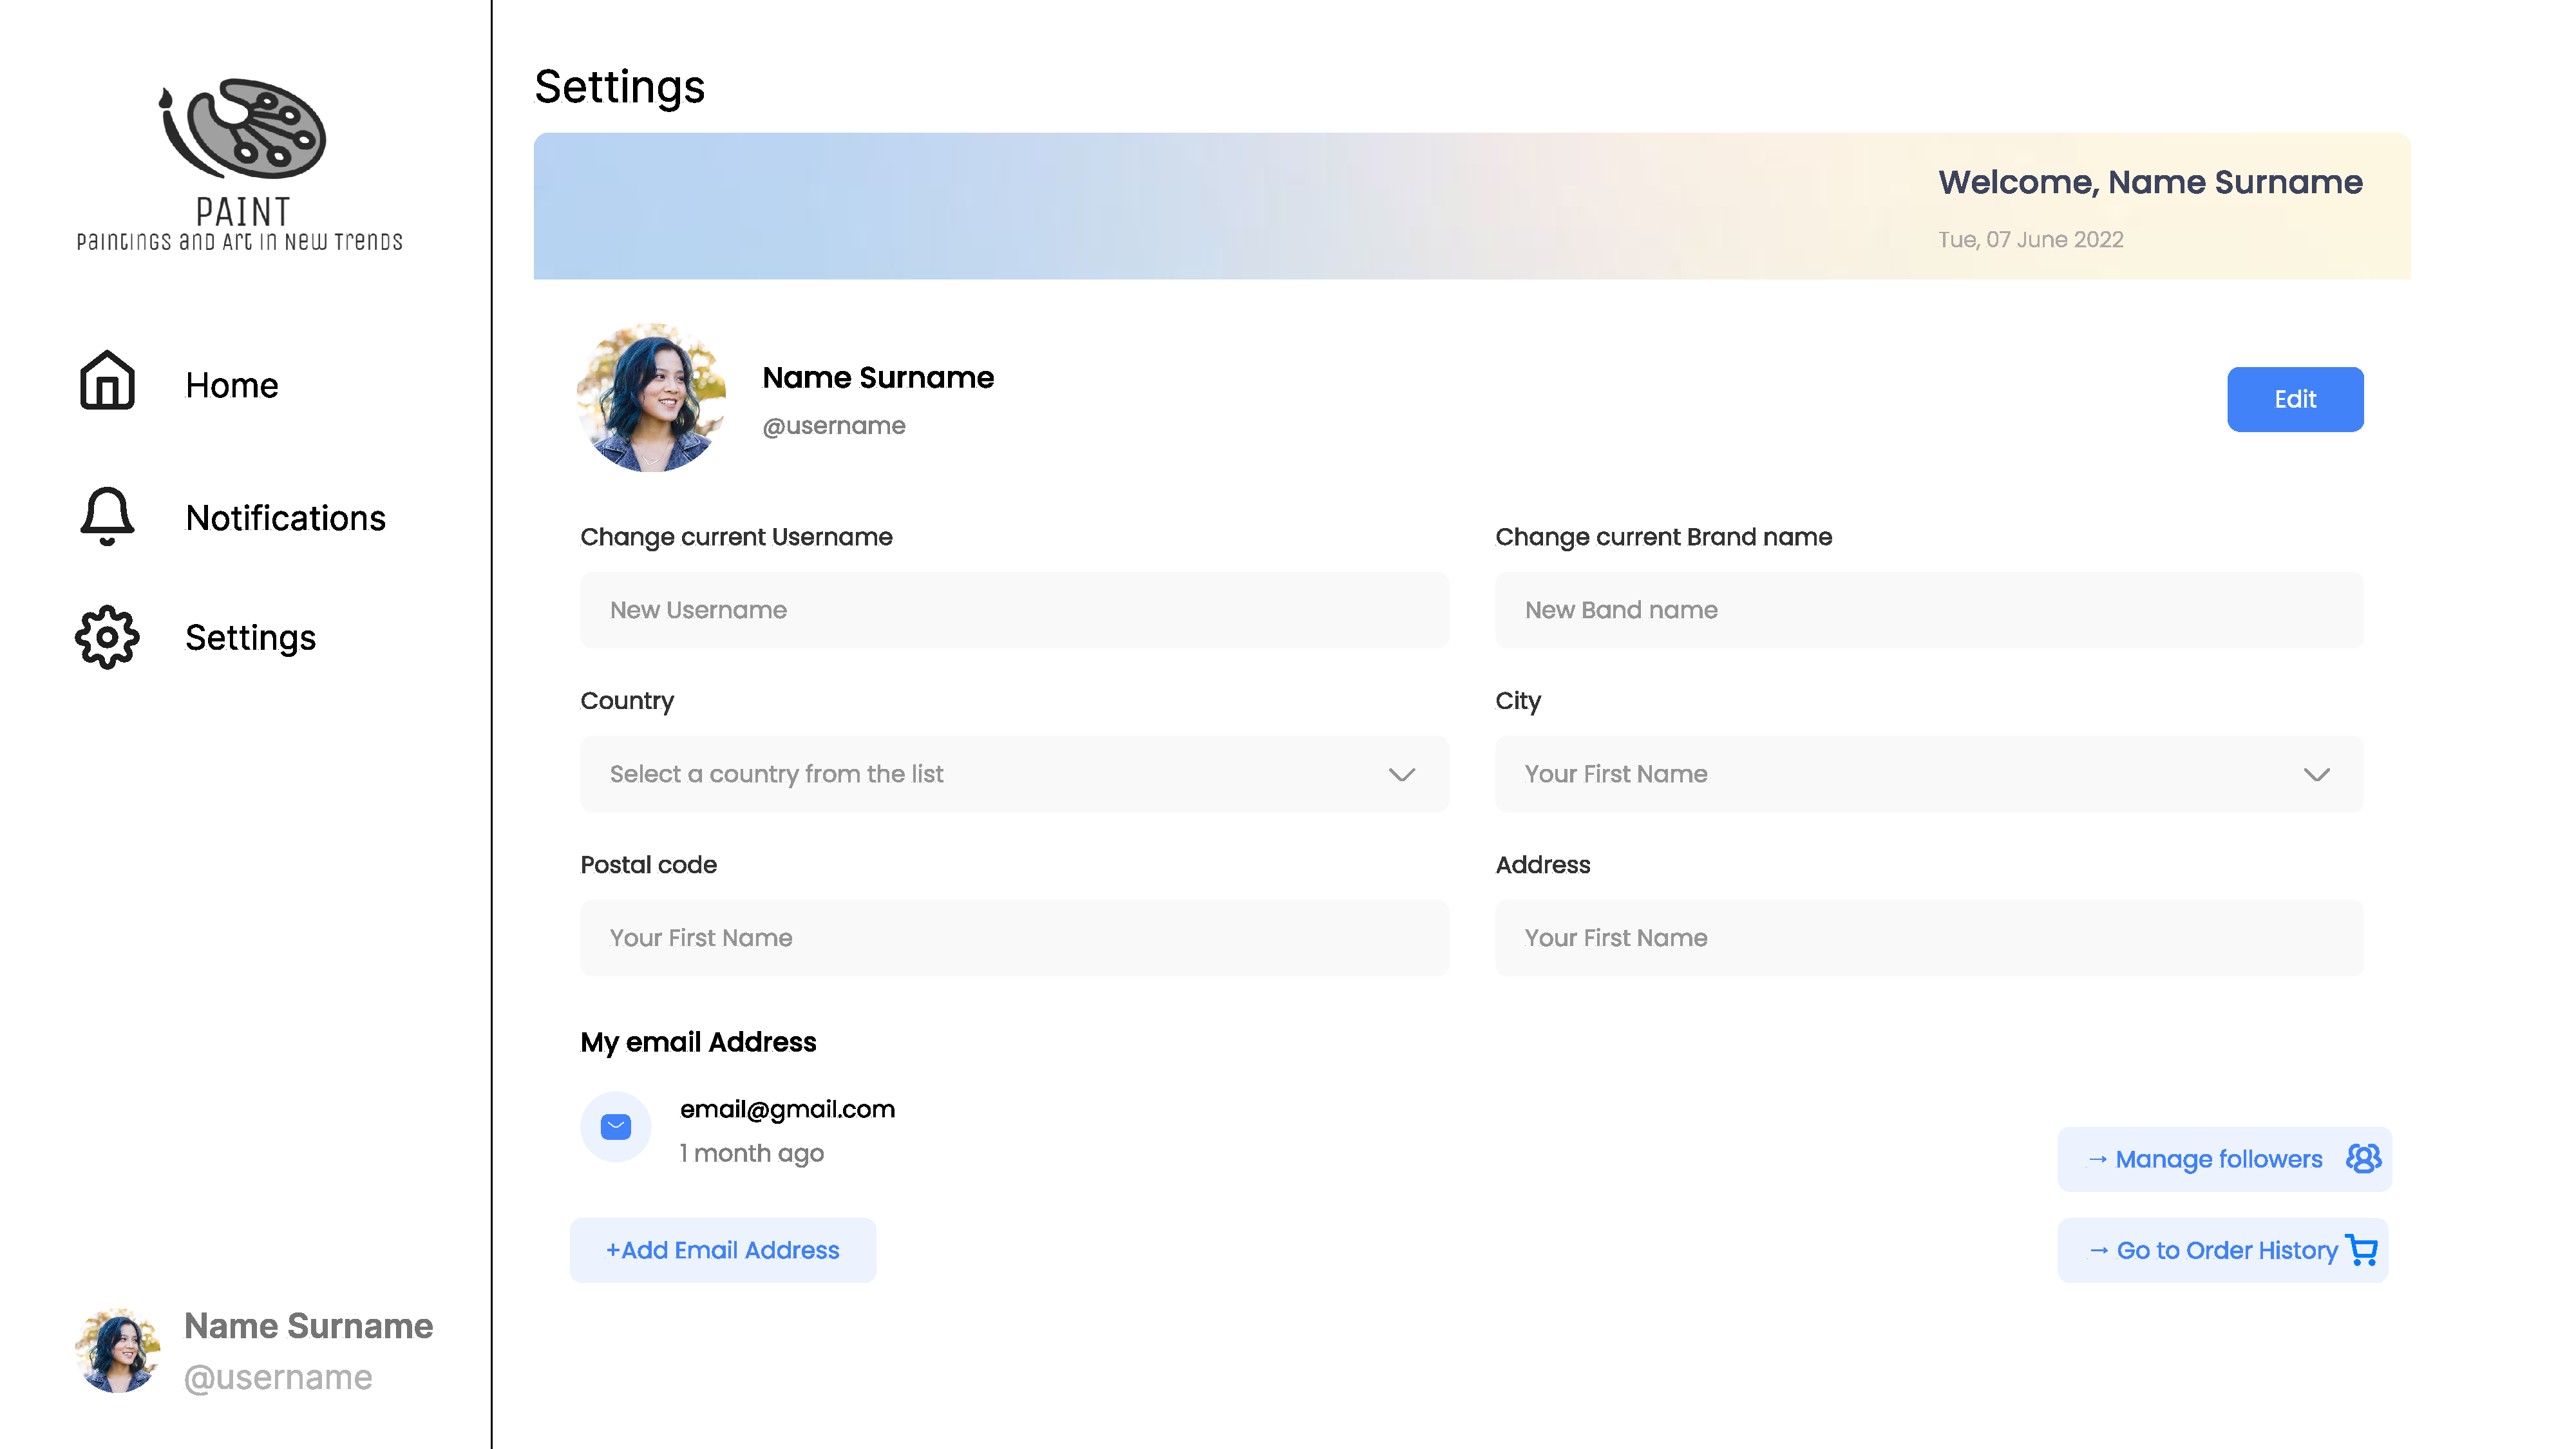
\includegraphics[width=\myfigwidth]{images/interface_mockups/Profile settings - main page.pdf}
    \caption{Profile settings main page}
\end{figure}

On the profile settings page, users can update their personal and account information. Additionally, they can navigate to their order history and the list of followed artists, each available on separate pages. The page ensures users maintain control over their preferences and past interactions.

%%%%%%%%%%%%%%%%%%%%%%%%%%%%%%%%%%%%%%%%%%%%%%%%%%%%%%%
\subsection{Artist profile page (Interface Mokup)}
\begin{figure}[H]
    \centering
\begin{subfigure}[b]{\myfigwidth}
    \centering
    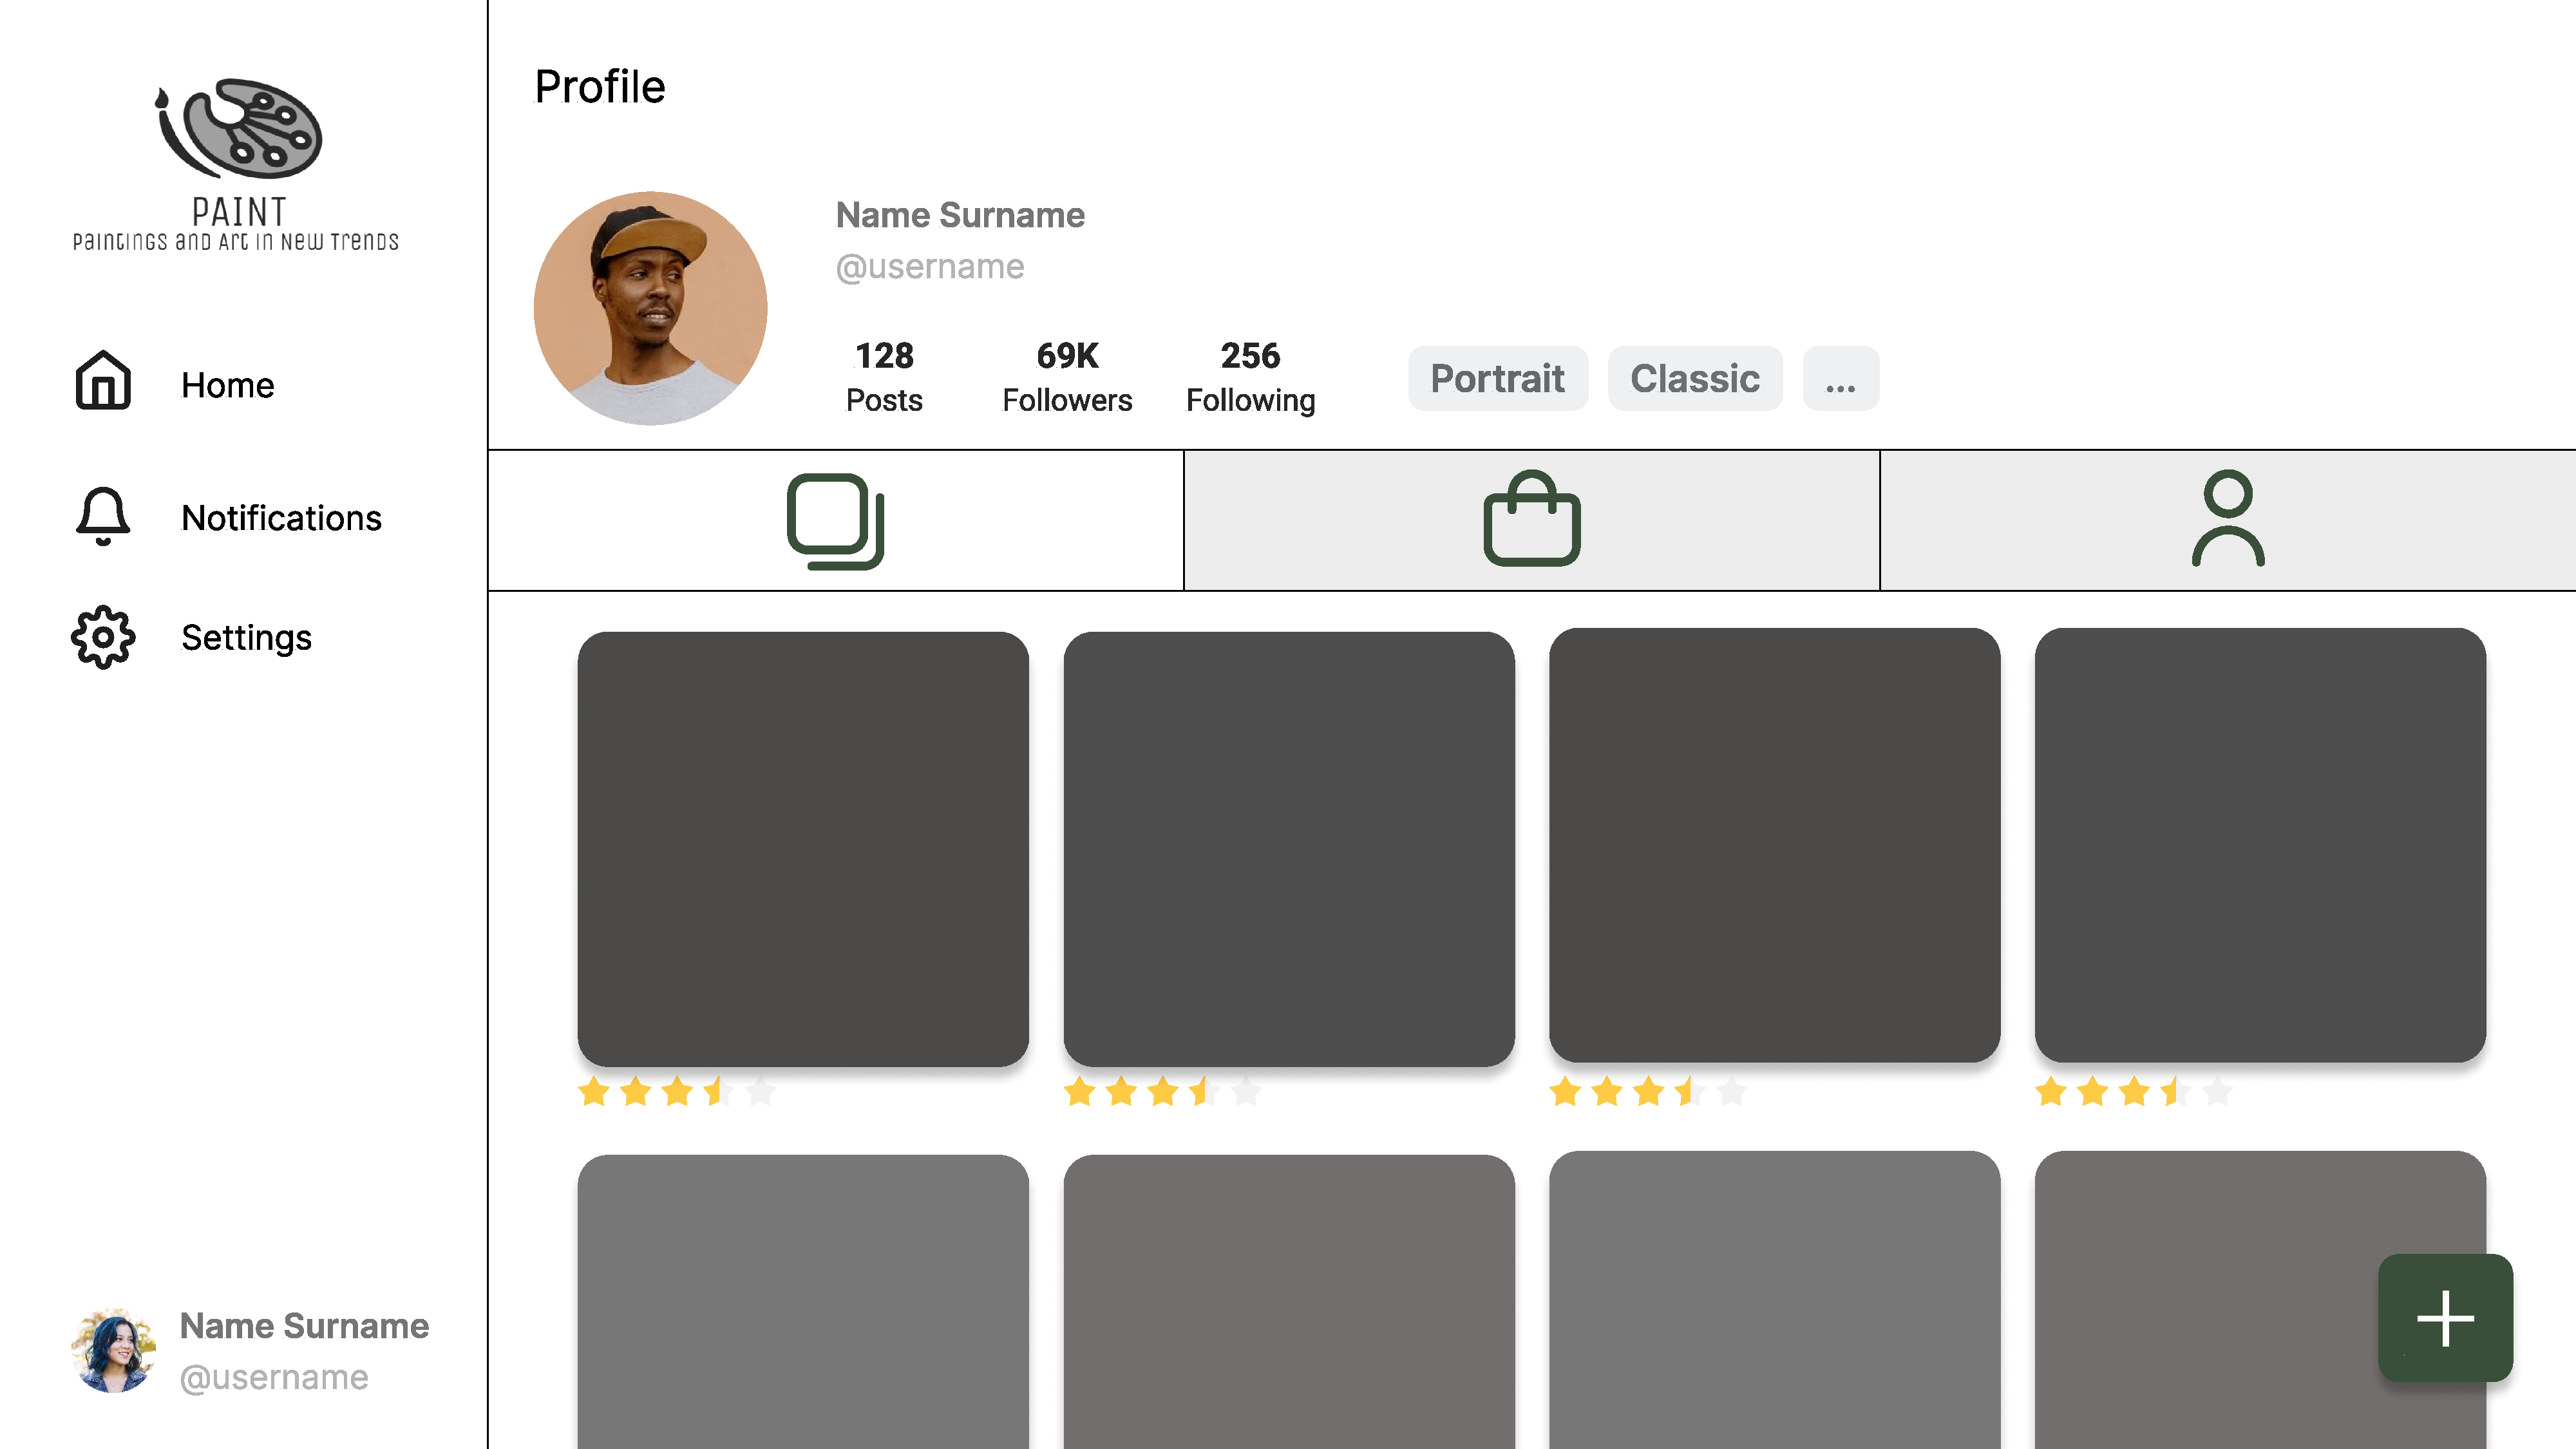
\includegraphics[width=\textwidth]{images/interface_mockups/Artist profile - showcase.pdf}
    \caption{Artpieces showcase page}
\end{subfigure}
\begin{subfigure}[b]{\myfigwidth}
    \centering
    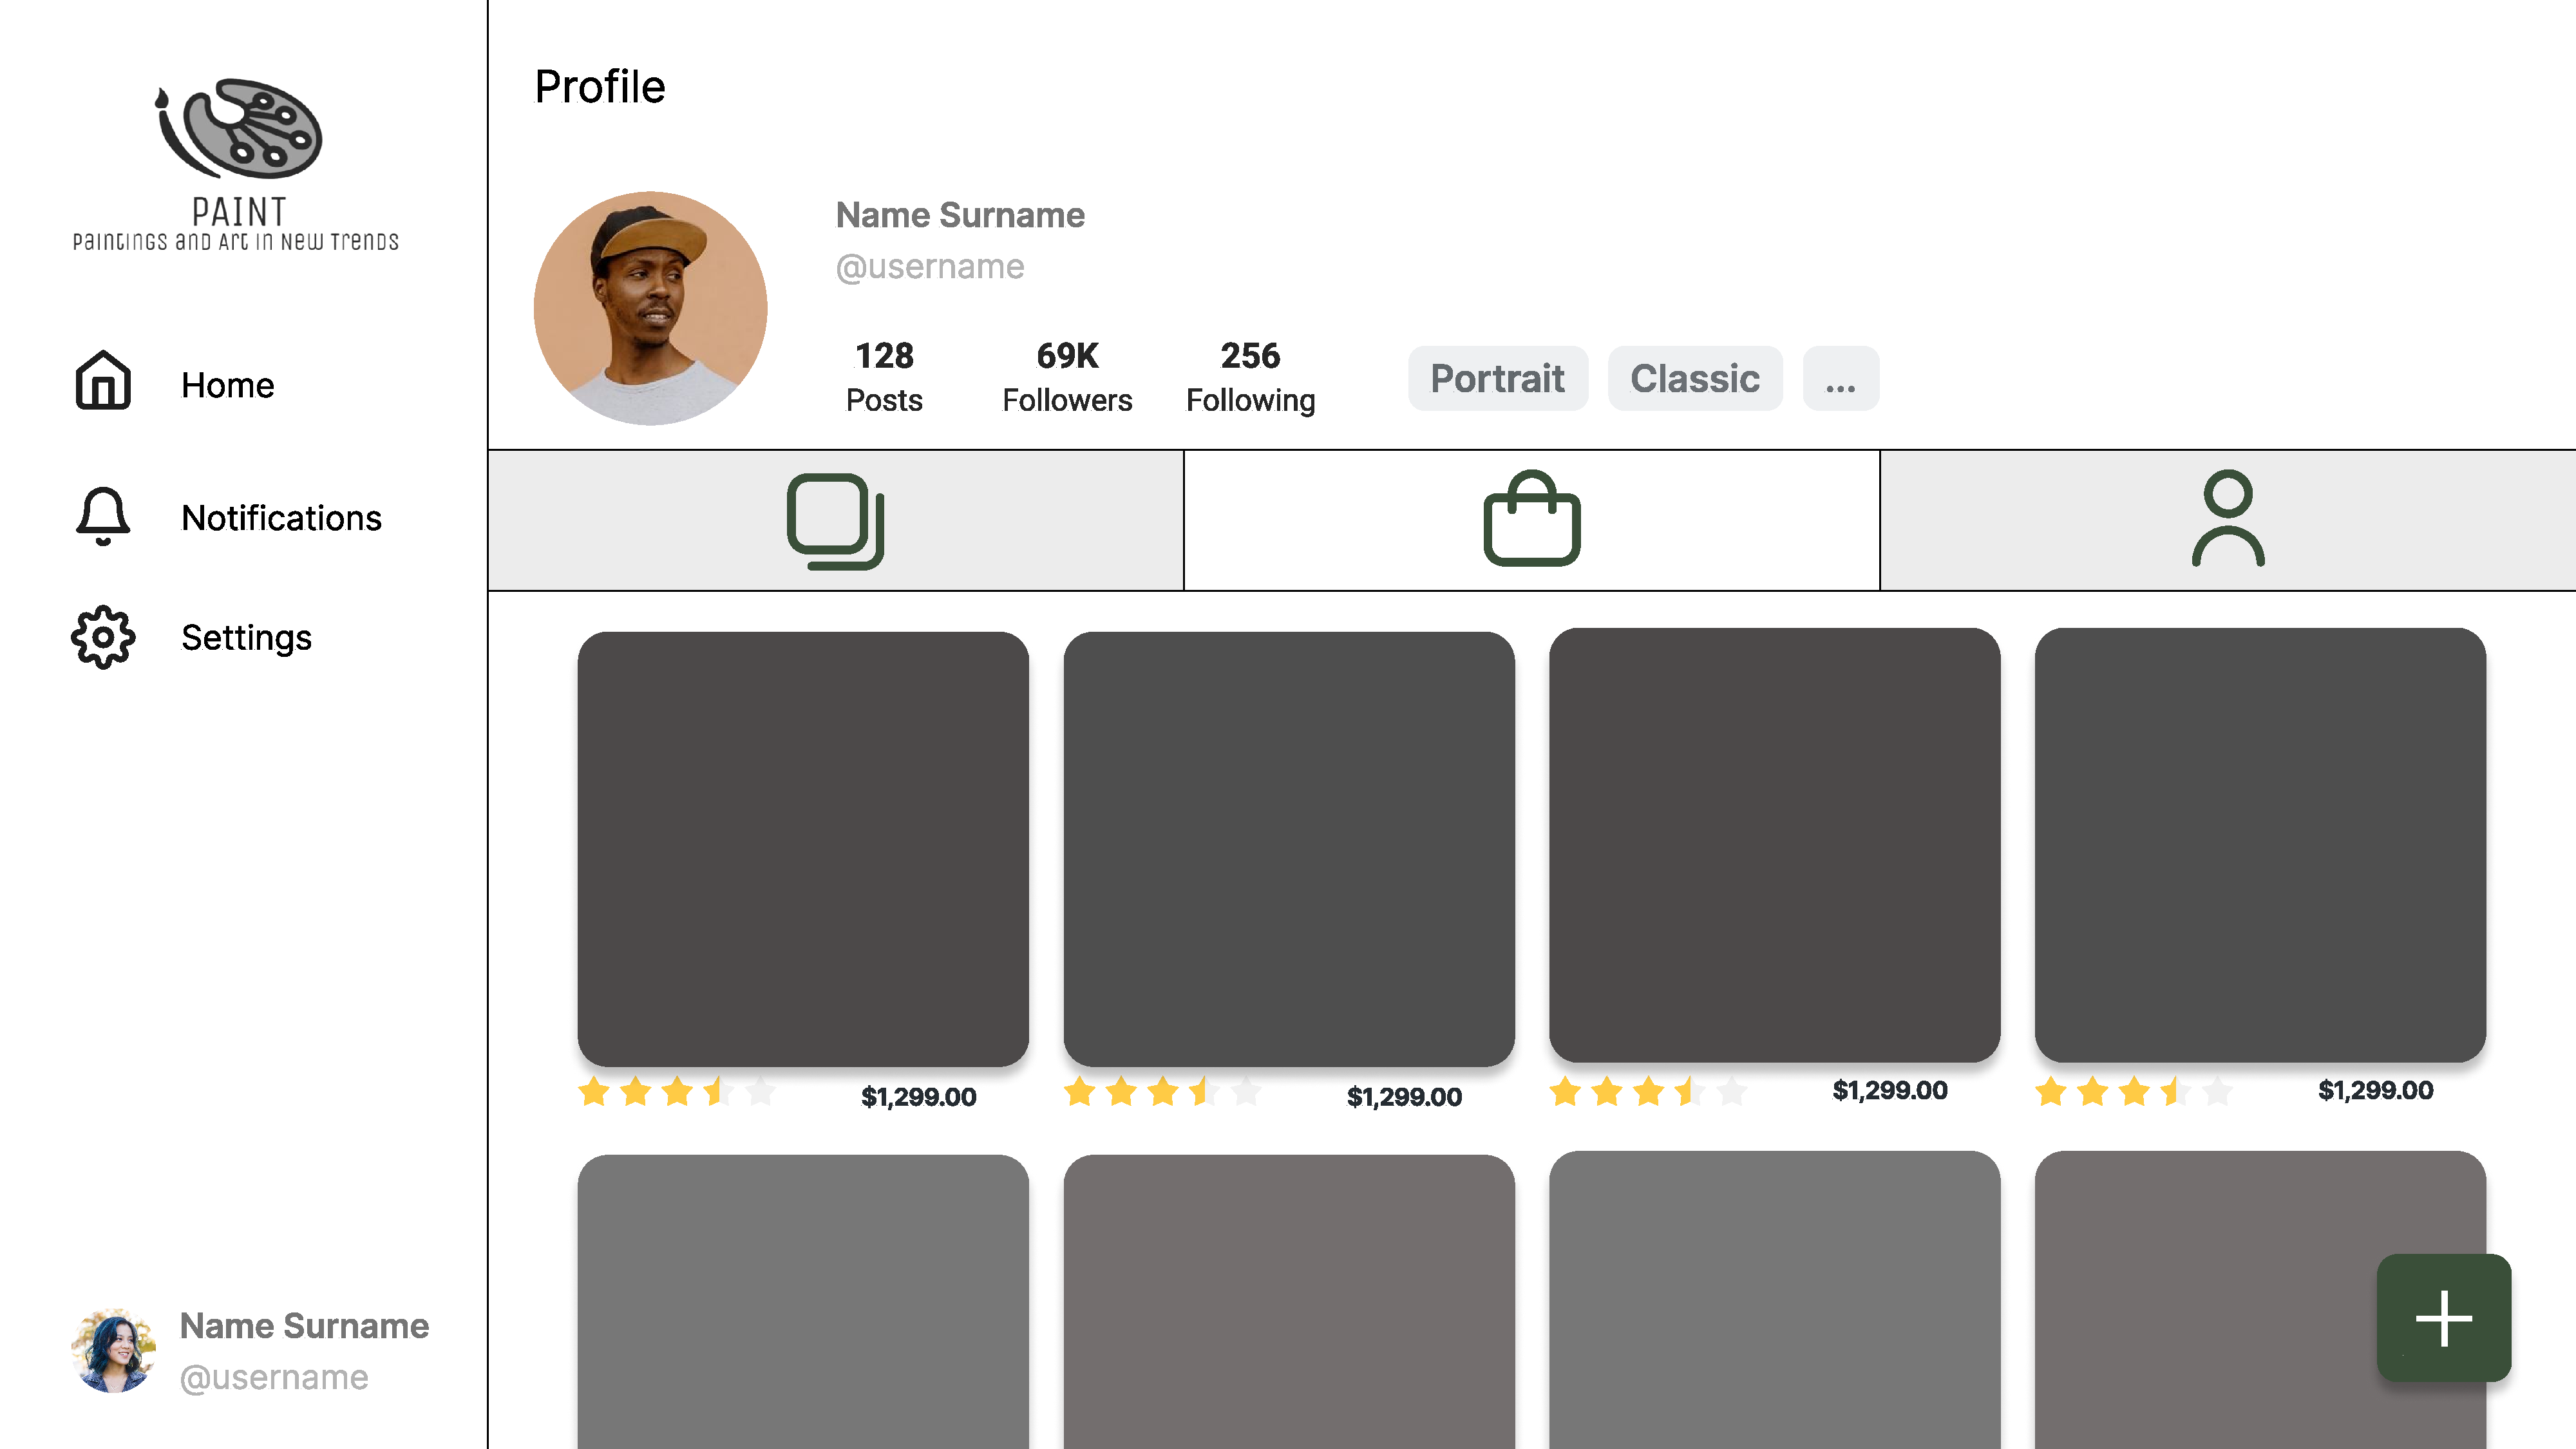
\includegraphics[width=\textwidth]{images/interface_mockups/Artist profile - shop.pdf}
    \caption{Shop section}
\end{subfigure}
\begin{subfigure}[b]{\myfigwidth}
    \centering
    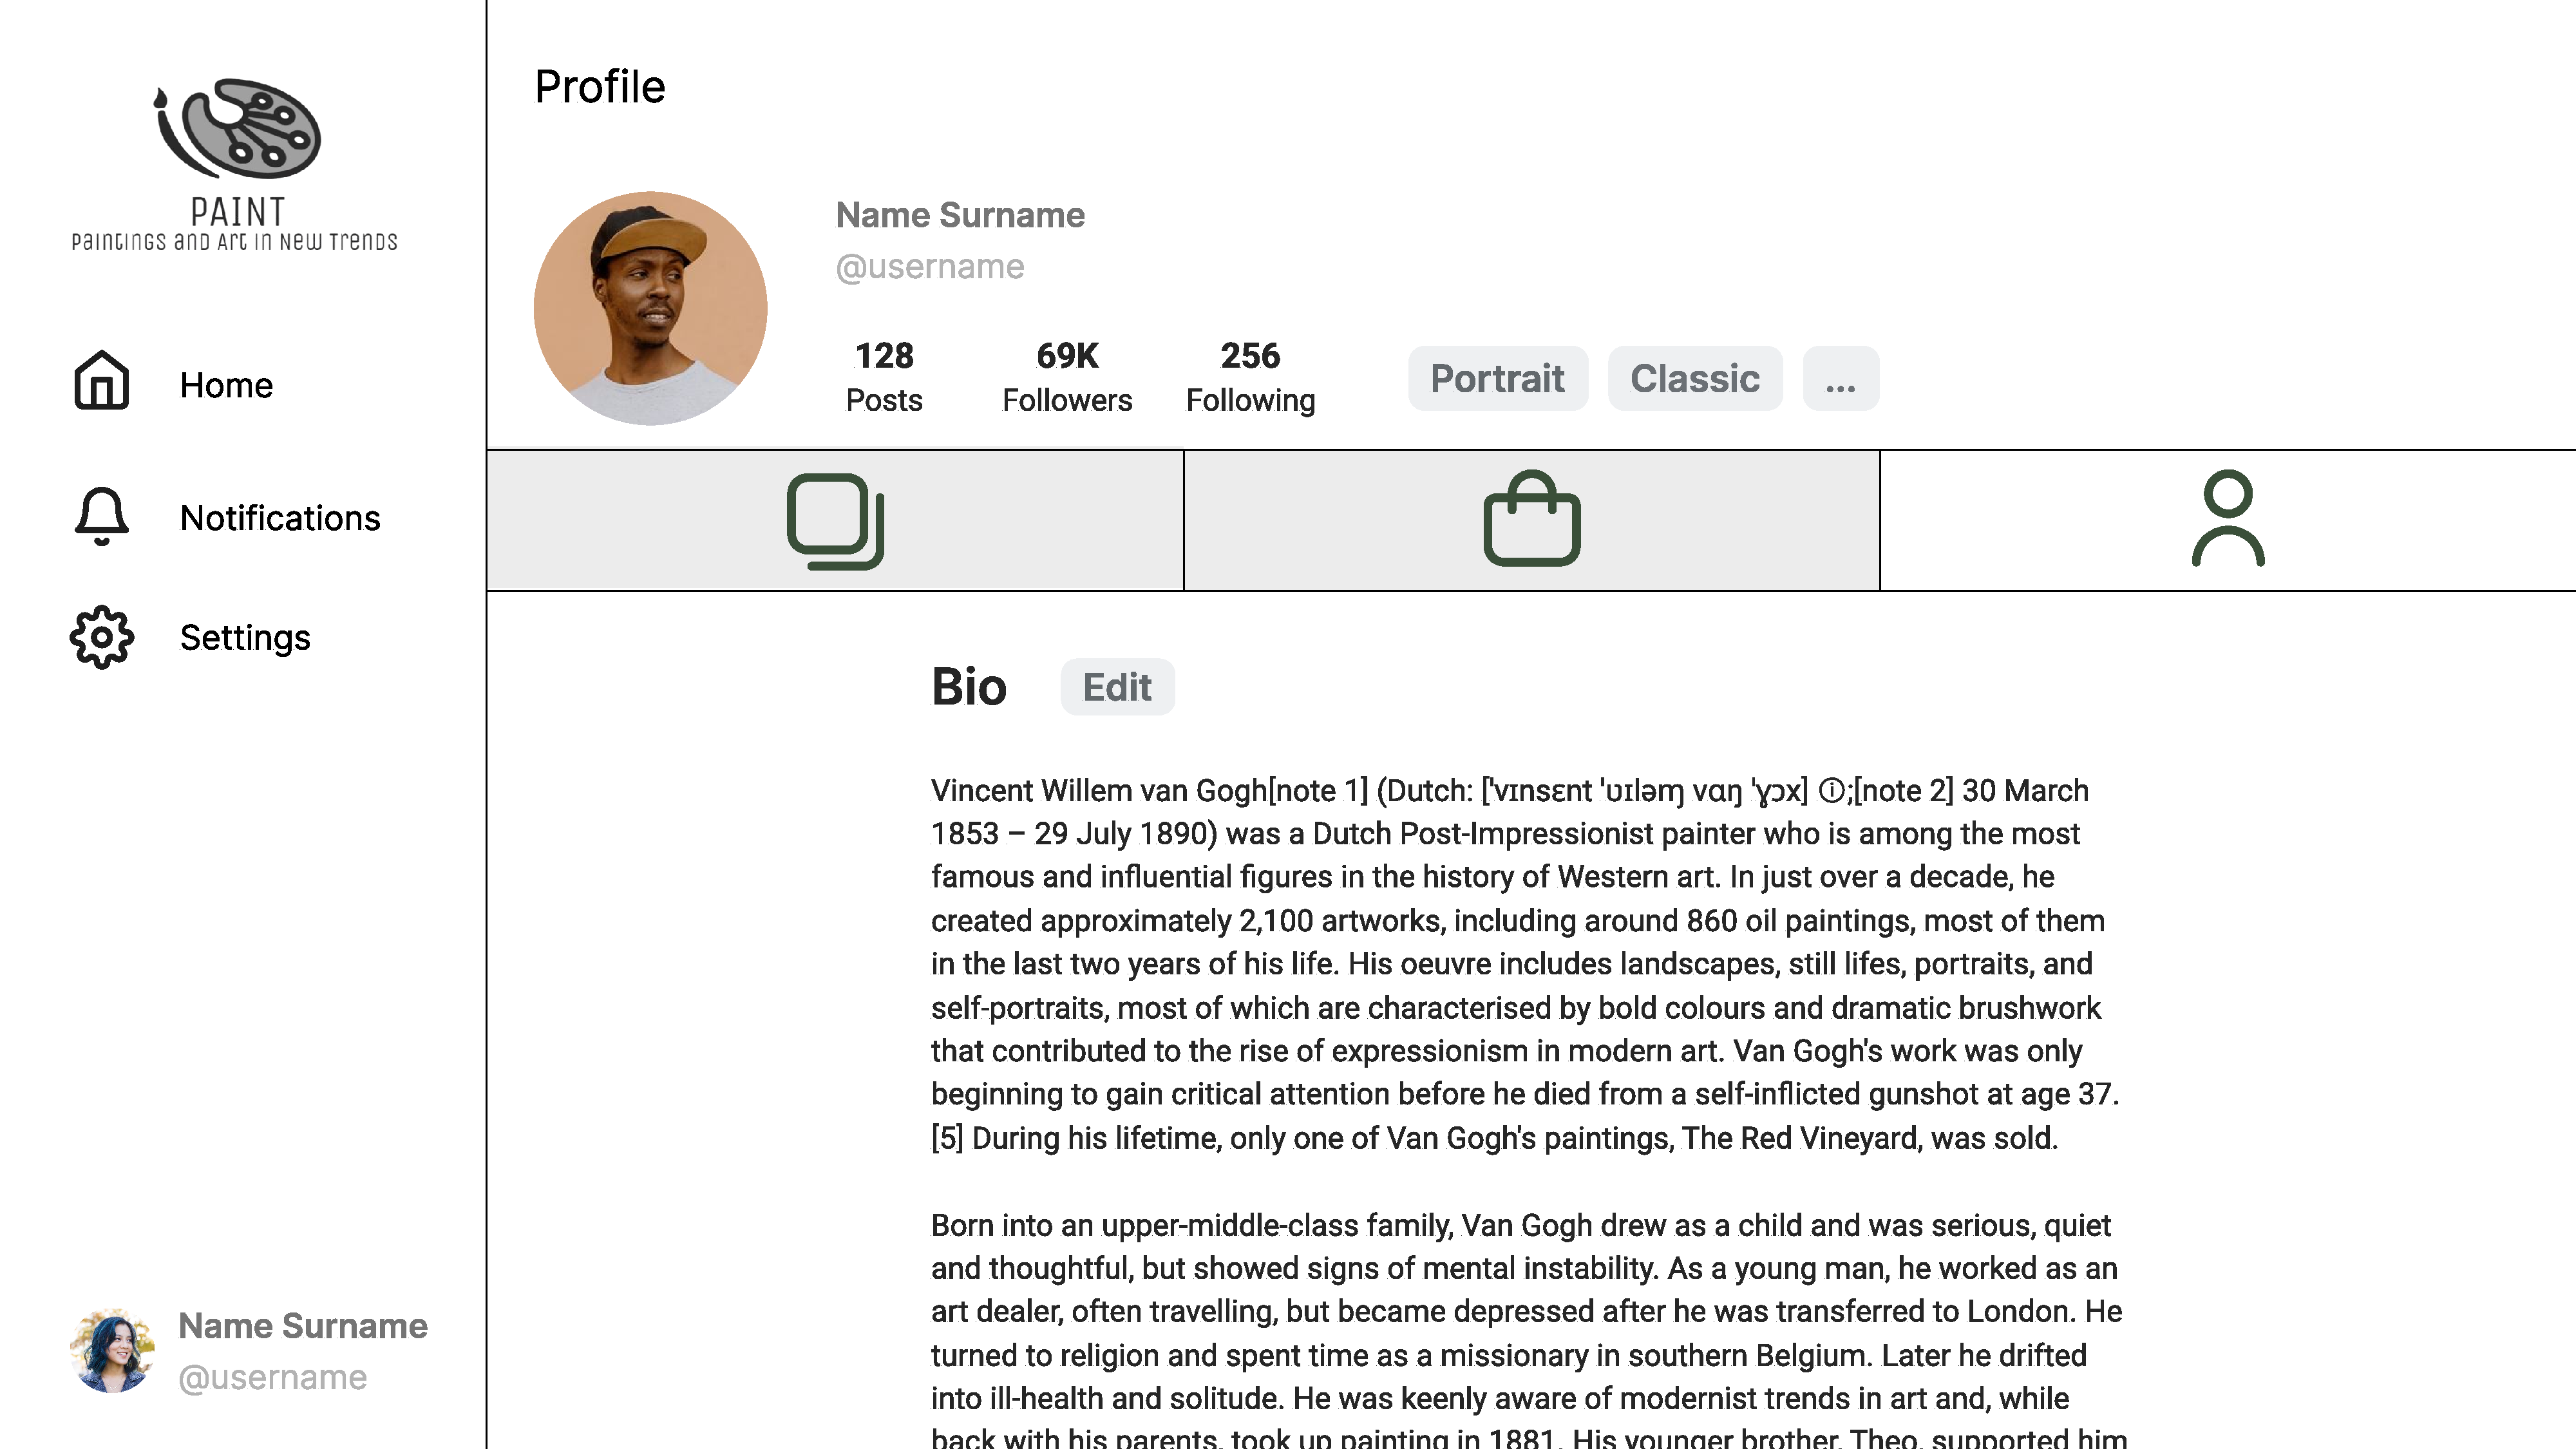
\includegraphics[width=\textwidth]{images/interface_mockups/Artist profile - bio.pdf}
    \caption{Artist biography page}
\end{subfigure}
\end{figure}

The artist profile page is a comprehensive space dedicated to presenting an artist’s work and personal narrative. 
It is divided into three main sections: the showcase section displays a complete gallery of the artist’s uploaded art pieces.
The shop section provides a streamlined interface for purchasing available art pieces, complete with pricing and transactional details; 
and the biography section offers an in-depth narrative of the artist’s background, influences, and career milestones.

%%%%%%%%%%%%%%%%%%%%%%%%%%%%%%%%%%%%%%%%%%%%%%%%%%%%%%%
\subsection{Art gallery profile page (Interface Mokup)}
\begin{figure}[H]
    \centering
\begin{subfigure}[b]{\myfigwidth}
    \centering
    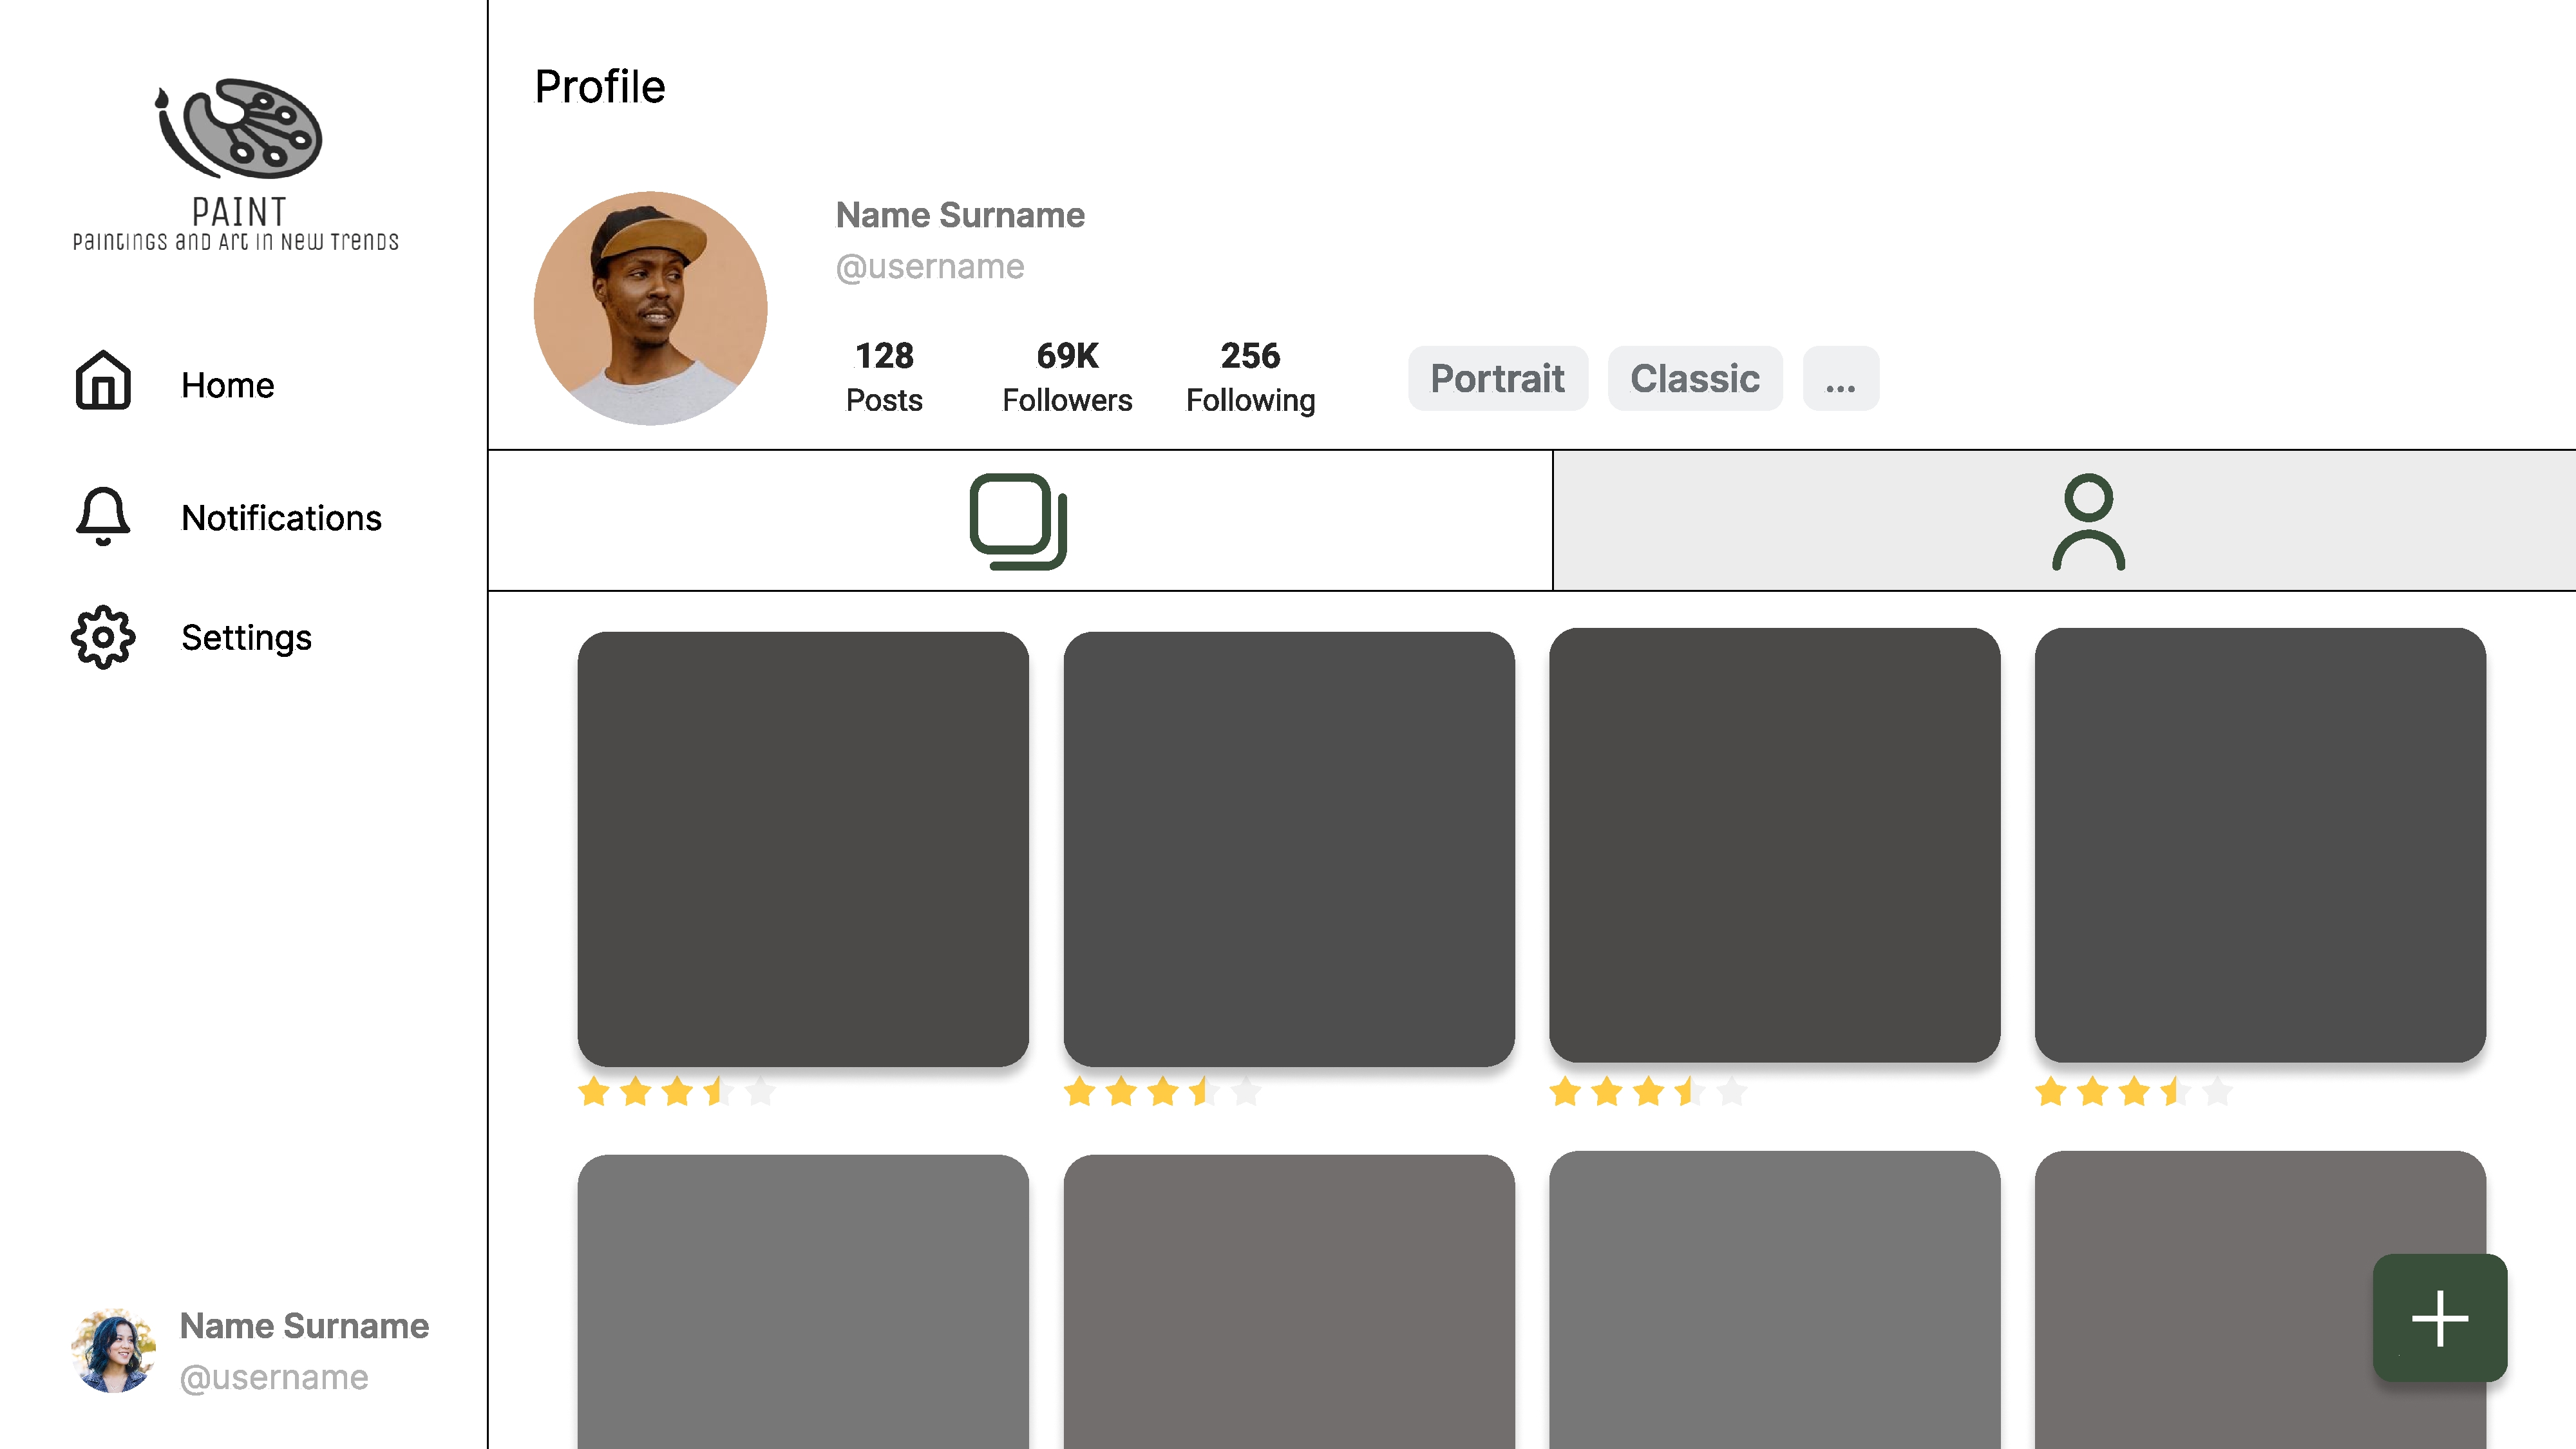
\includegraphics[width=\textwidth]{images/interface_mockups/Art gallery profile - showcase.pdf}
    \caption{Art gallery showcase page}
\end{subfigure}
\begin{subfigure}[b]{\myfigwidth}
    \centering
    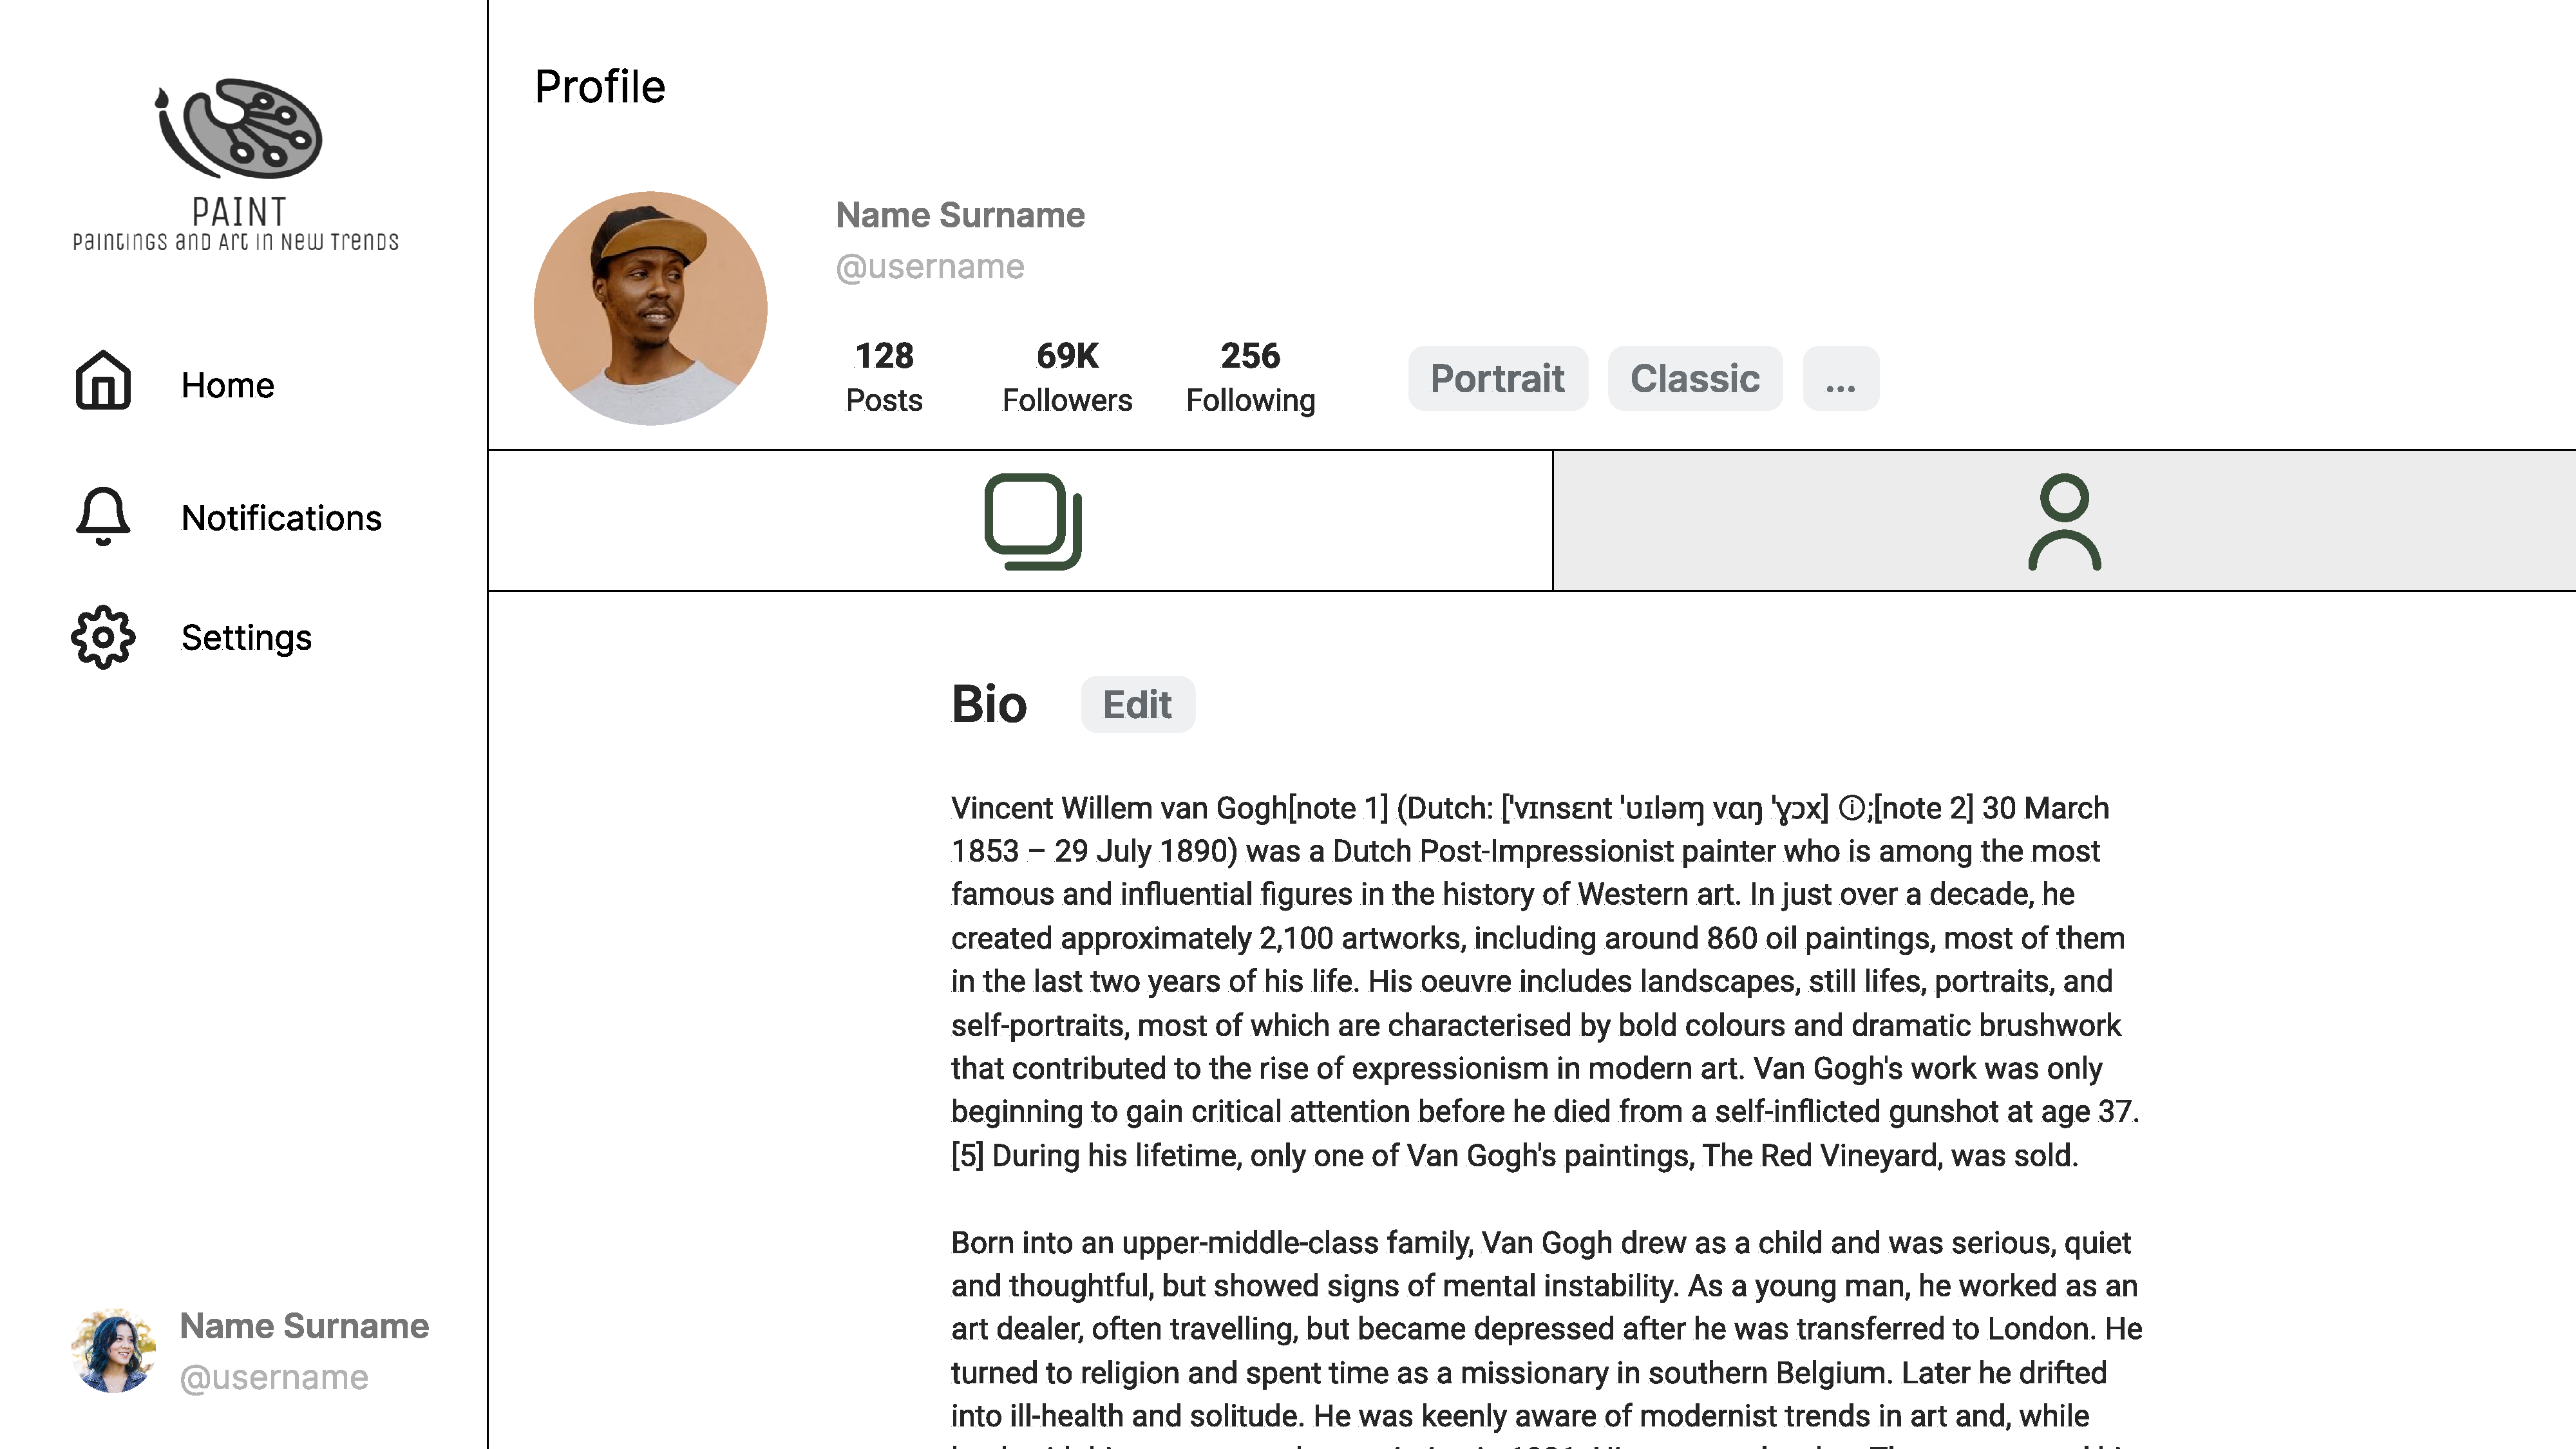
\includegraphics[width=\textwidth]{images/interface_mockups/Art gallery profile - bio.pdf}
    \caption{Art gallery biography page}
\end{subfigure}
\end{figure}

The art gallery profile page is structured to present the gallery’s events and background information. 
It comprises two primary sections: the showcase section highlights current and past events hosted by the gallery; the biography section provides a detailed account of the gallery’s history, mission, and artistic curatorial approach.

%%%%%%%%%%%%%%%%%%%%%%%%%%%%%%%%%%%%%%%%%%%%%%%%%%%%%%%
\subsection{Art piece page (Interface Mokup)}
\begin{figure}[H]
    \centering
    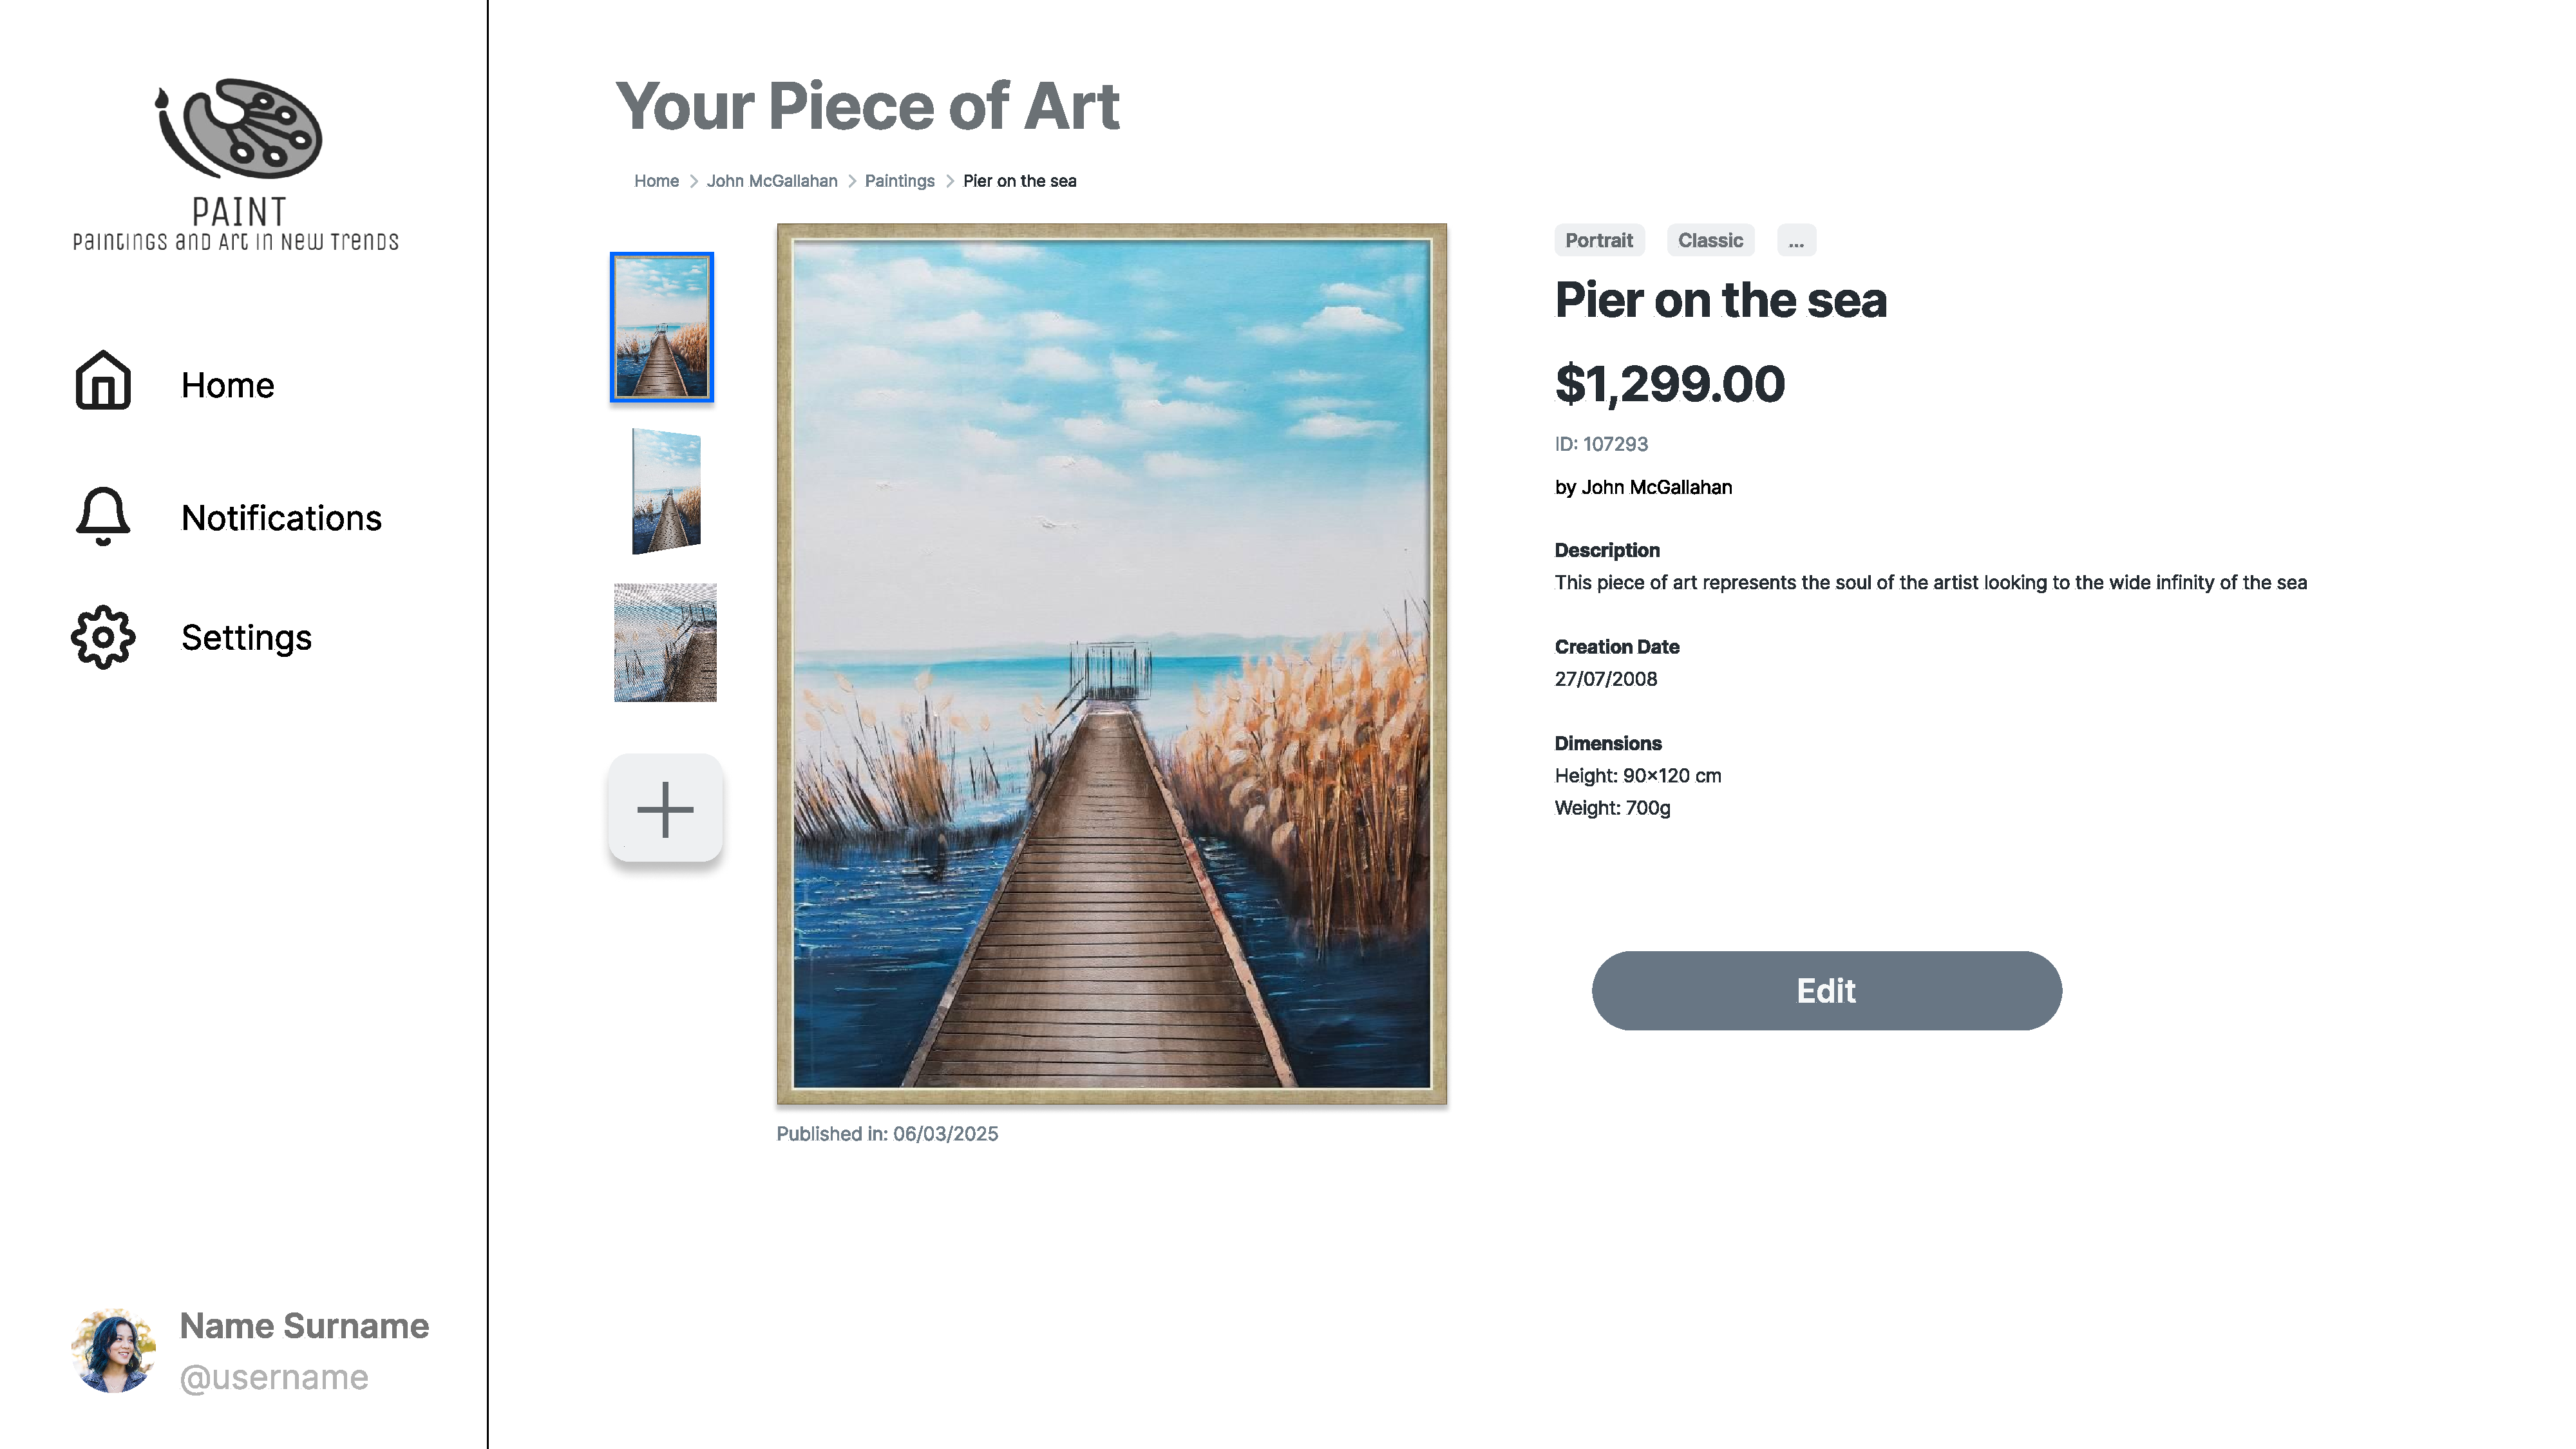
\includegraphics[width=\myfigwidth]{images/interface_mockups/Art piece page.pdf}
    \caption{Art piece page}
\end{figure}

The art piece page delivers an in-depth view of individual artworks, presenting key details such as the title, artist information, creation date, dimensions, weight and description. 
If the artwork is available for sale, the page displays its price and includes an option to proceed with a purchase, leading the user to the order page. 
Its design emphasizes clarity, ensuring that potential buyers have all necessary information.

%%%%%%%%%%%%%%%%%%%%%%%%%%%%%%%%%%%%%%%%%%%%%%%%%%%%%%%
\subsection{Order page (Interface Mokup)}
\begin{figure}[H]
    \centering
    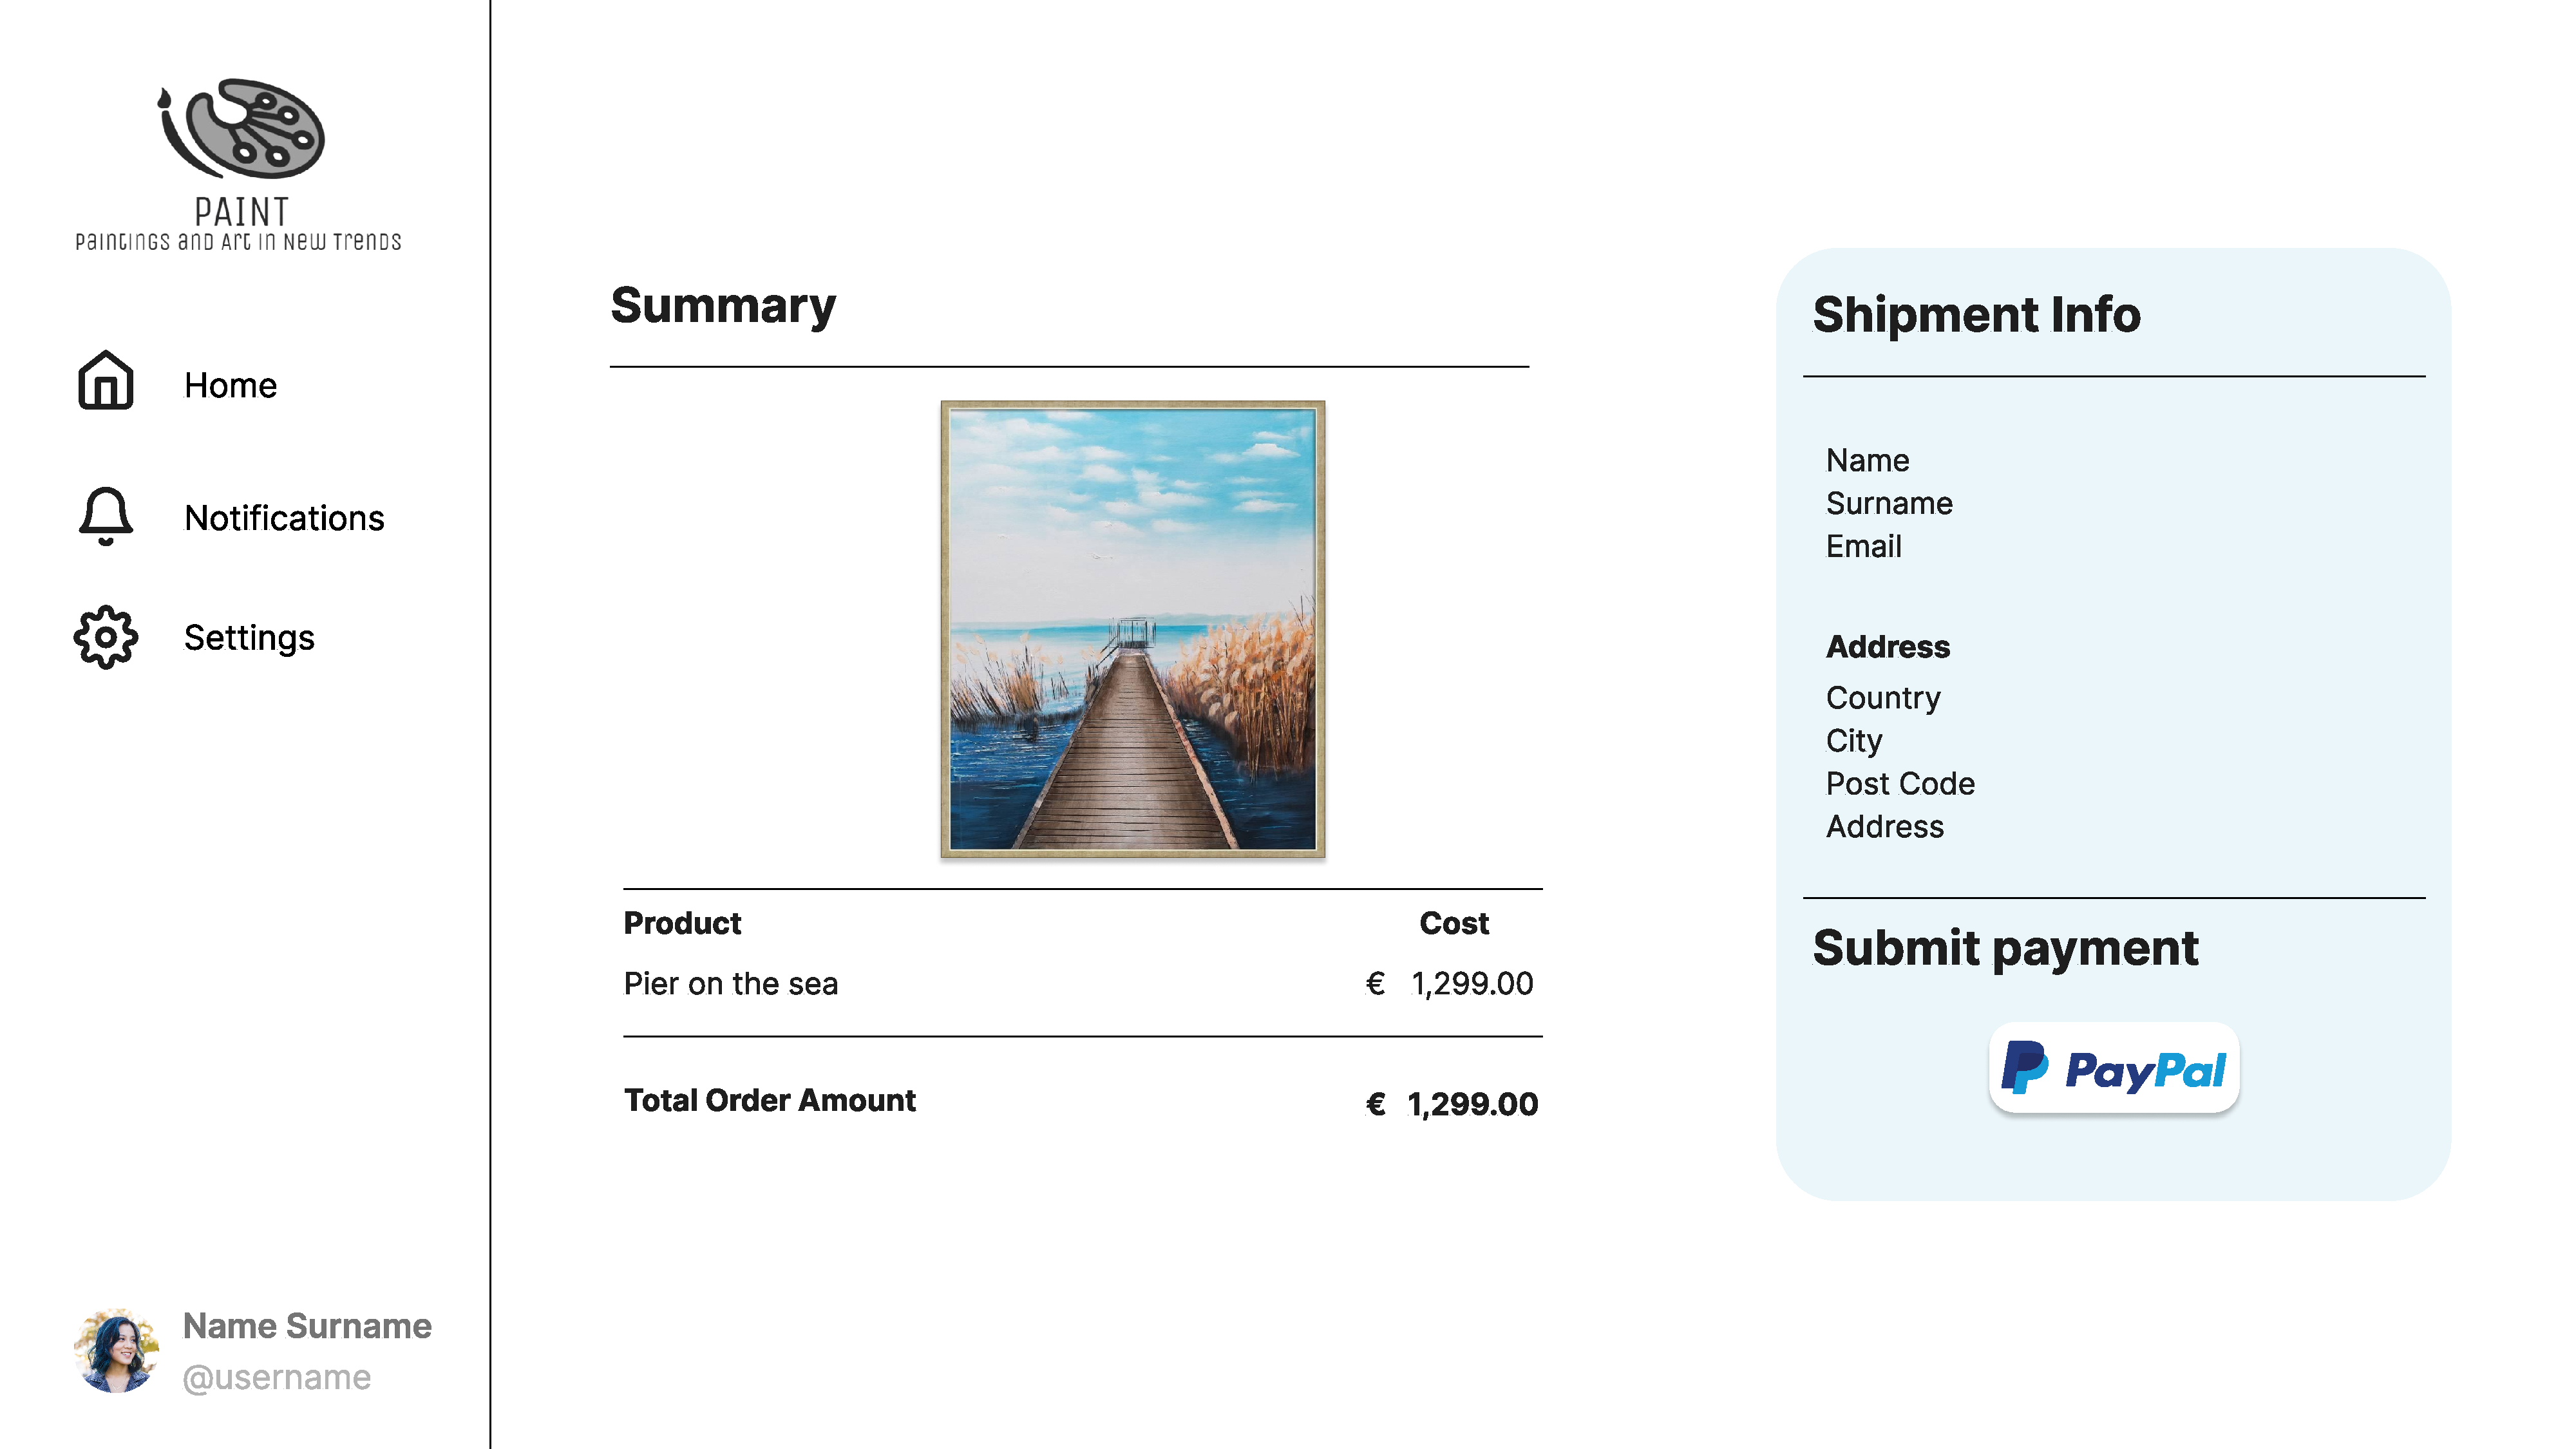
\includegraphics[width=\myfigwidth]{images/interface_mockups/Order page.pdf}
    \caption{Order page}
\end{figure}

On the order page, users can review their purchase details, including the selected art piece and its cost. They must provide shipping information such as name, surname, email, country, city, postal code, and address. After reviewing the total order amount, users can proceed with the payment using their PayPal account.

%%%%%%%%%%%%%%%%%%%%%%%%%%%%%%%%%%%%%%%%%%%%%%%%%%%%%%%
\subsection{Order history page (Interface Mokup)}
\begin{figure}[H]
    \centering
    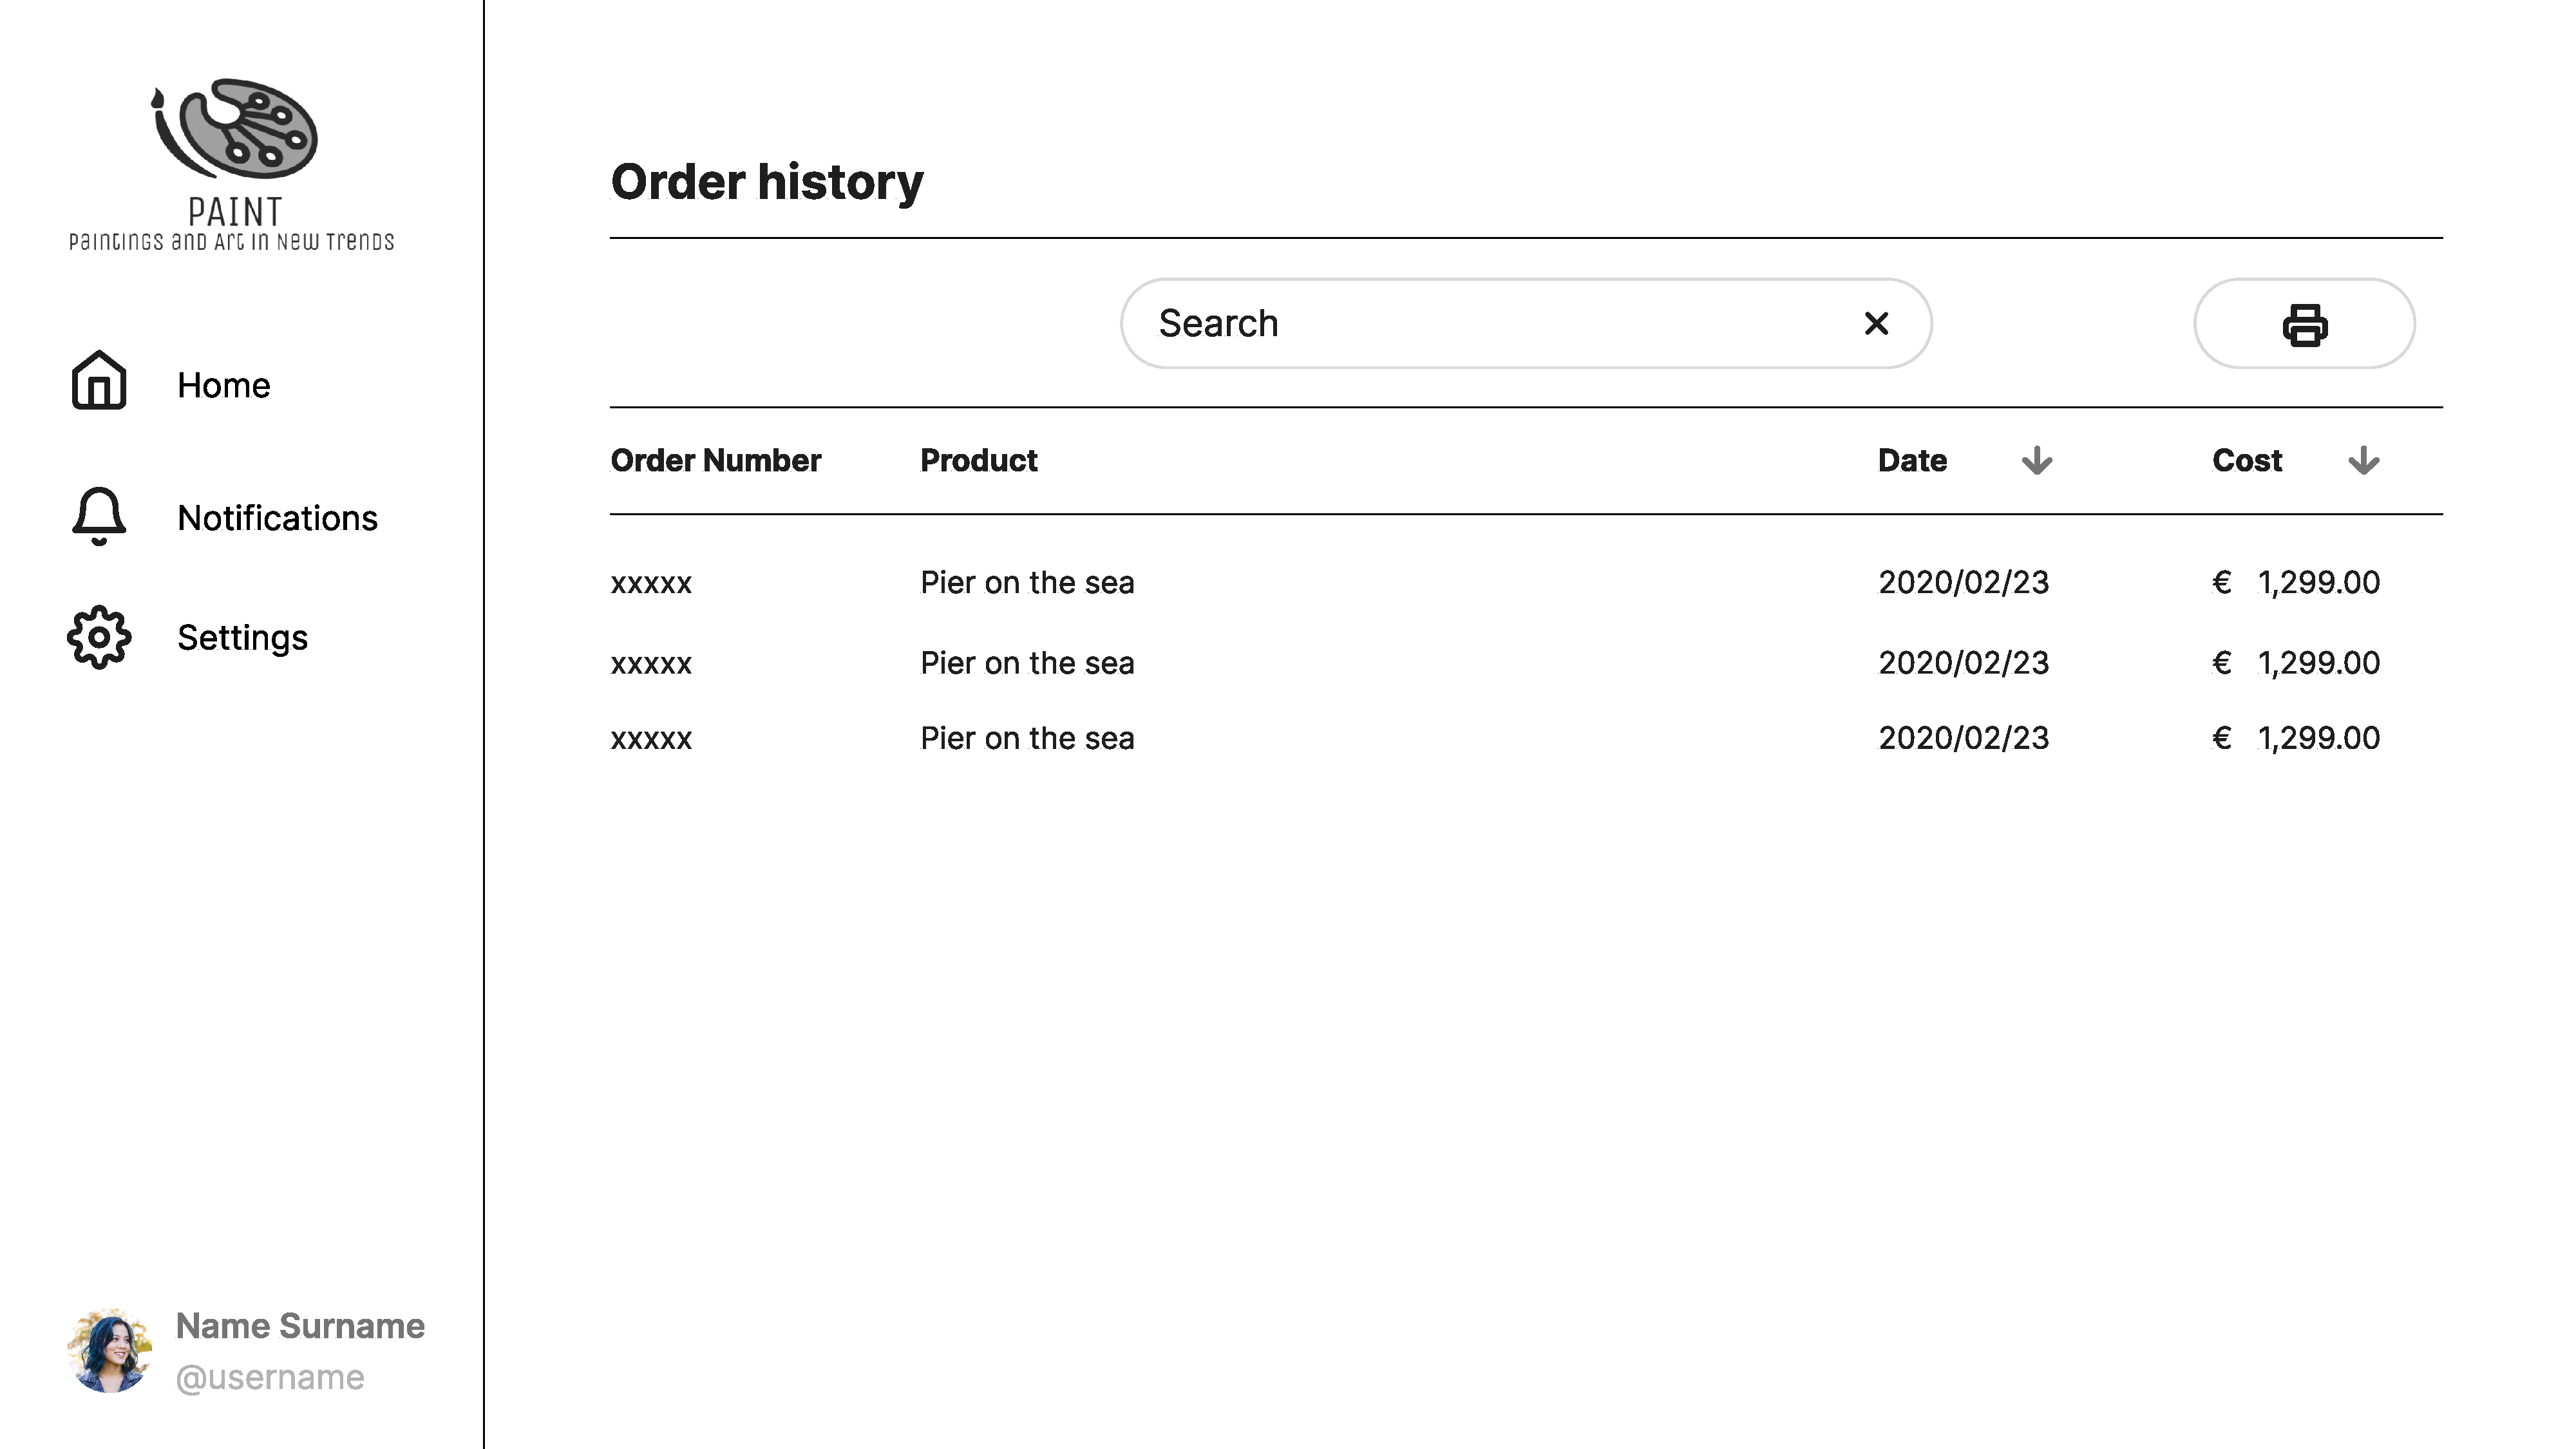
\includegraphics[width=\myfigwidth]{images/interface_mockups/Order History.pdf}
    \caption{Order history page}
\end{figure}

The order history page provides a comprehensive log of all transactions completed by the user. It organizes past orders in a chronological format, with each entry detailing the order number, purchase date, product name, and cost. Users are afforded the option to filter and sort their order history by date or cost. 
The page ensures users can easily track their transactions and retrieve information about previous purchases.